\documentclass{article}

% if you need to pass options to natbib, use, e.g.:
\PassOptionsToPackage{square, authoryear, comma, sort&compress}{natbib}
% before loading nips_2016
%
% to avoid loading the natbib package, add option nonatbib:
% \usepackage[nonatbib]{nips_2016}

\usepackage[final]{nips_2016}

% to compile a camera-ready version, add the [final] option, e.g.:
% \usepackage[final]{nips_2016}

\usepackage[utf8x]{inputenc} % allow utf-8 input
\usepackage[T1]{fontenc}    % use 8-bit T1 fonts
\usepackage[colorlinks=true,linkcolor=green,citecolor=cyan]{hyperref}       % hyperlinks
\usepackage{url}            % simple URL typesetting
\usepackage{booktabs}       % professional-quality tables
\usepackage{amsfonts}       % blackboard math symbols
\usepackage{nicefrac}       % compact symbols for 1/2, etc.
\usepackage{microtype}      % microtypography

% My Packages
\usepackage{amsmath}
\usepackage{amssymb}
\usepackage{amsthm}
\usepackage{mathbbol}
\usepackage{mathtools}
\usepackage{mathrsfs}
\usepackage{vector}
\usepackage{cleveref}
\usepackage{bm}
\usepackage[dvipsnames]{xcolor}

\newcommand{\argmax}{\operatornamewithlimits{argmax}}
\newcommand{\note}[1]{{\color{orange} #1}}
\newcommand{\edit}[1]{{\color{forestgreen} #1}}

\newtheorem{theorem}{Theorem}[section]
\newtheorem{corollary}[theorem]{Corollary}
\newtheorem{lemma}[theorem]{Lemma}
\newtheorem{claim}[theorem]{Claim}

\usepackage{multirow}

\usepackage{algorithm}
\usepackage{algorithmic}

\title{CAKE: Classification avec Kernel Embeddings \\ with Rademacher Complexity Bounds}

% The \author macro works with any number of authors. There are two
% commands used to separate the names and addresses of multiple
% authors: \And and \AND.
%
% Using \And between authors leaves it to LaTeX to determine where to
% break the lines. Using \AND forces a line break at that point. So,
% if LaTeX puts 3 of 4 authors names on the first line, and the last
% on the second line, try using \AND instead of \And before the third
% author name.

%\author{
%  Kelvin Y.S. Hsu, Richard Nock, Fabio T. Ramos \\
%  University of Sydney, Australia\\
%  DATA61, CSIRO\\
%  \texttt{\{Kelvin.Hsu, Richard.Nock, Fabio.Ramos\}@\{sydney.edu.au, data61.csiro.au\}} \\
%  %% examples of more authors
%  %% \And
%  %% Coauthor \\
%  %% Affiliation \\
%  %% Address \\
%  %% \texttt{email} \\
%  %% \AND
%  %% Coauthor \\
%  %% Affiliation \\
%  %% Address \\
%  %% \texttt{email} \\
%  %% \And
%  %% Coauthor \\
%  %% Affiliation \\
%  %% Address \\
%  %% \texttt{email} \\
%  %% \And
%  %% Coauthor \\
%  %% Affiliation \\
%  %% Address \\
%  %% \texttt{email} \\
%}

\author{
	Kelvin Y.S. Hsu \\
	University of Sydney, Australia\\
	DATA61, CSIRO\\
	\texttt{Kelvin.Hsu@\{sydney.edu.au, data61.csiro.au\}} \\
	%% examples of more authors
	\And
	Richard Nock \\
	Australian National University, Australia\\
	University of Sydney, Australia\\
	DATA61, CSIRO\\
	\texttt{Richard.Nock@data61.csiro.au} \\
	\And
	Fabio T. Ramos \\
	University of Sydney, Australia\\
	DATA61, CSIRO\\
	\texttt{Fabio.Ramos@\{sydney.edu.au, data61.csiro.au\}} \\
	%% \texttt{email} \\
	%% \AND
	%% Coauthor \\
	%% Affiliation \\
	%% Address \\
	%% \texttt{email} \\
	%% \And
	%% Coauthor \\
	%% Affiliation \\
	%% Address \\
	%% \texttt{email} \\
	%% \And
	%% Coauthor \\
	%% Affiliation \\
	%% Address \\
	%% \texttt{email} \\
}

\begin{document}


\maketitle

\begin{abstract}
	We propose learning-theoretic bounds for learning the hyperparameters of kernel embeddings in the probabilistic multiclass classification context. Kernel embeddings are nonparametric methods to represent probability distributions directly through observed data in a reproducing kernel Hilbert space (RKHS). However, the problem of hyperparameter learning for kernel embeddings remains challenging, often relying on heuristics and domain specific knowledge. We begin by developing the kernel embedding classifier (KEC), and prove the stochastic convergence of its probabilistic predictions. We then prove that expected classification risk can be bounded by using a data dependent Rademacher complexity measure in the probably approximately correct (PAC) framework. We use this bound to propose a scalable kernel learning algorithm for probabilistic multiclass classification. Classification performance is benchmarked on standard UCI datasets. We further apply our proposed kernel learning algorithm to learn feature representations of a deep convolutional network, with improved accuracy as compared to the original network, demonstrating the generality of this approach.
\end{abstract}

- We address the need for a principled way of obtaining probabilistic outputs from a multiclass classifier.
- It works in domains with not a lot of data, and we later provide a way for which it can scale
- We address hyperparameter learning for a kernel embedding model
- We do not rely on priors


Data dependent risk bounds
\section{Introduction}
\label{sec:introduction}
	
	Kernel embeddings are a principled way to represent probability distributions in a nonparametric setting.
	
	learning theoretic (be specific and mention PAC)
	(complexity penalty terms that are not data dependent cannot be universally effective) \citep{kearns1997experimental} 
	
	Classification is perhaps one of the most important and thoroughly developed topics in machine learning and pattern recognition. Despite this, principled probabilistic classification on multiclass problems remains a difficult and challenging task, and most solutions tackle this issue rather indirectly. \note{Maybe elaborate on why multiclass problems are important and why we want probabilities estimates in our predictions.}
	
	Support vector classifiers (SVC) \citep{m2001introduction}, for example, are originally designed for non-probabilistic binary classification. Its simple and convex optimisation structure makes the model very attractive both theoretically and in practice. However, in order to cope with overfitting, slack constraints introduce hyperparameters for which training does not directly addressed except through standard cross-validation. In order to extend to multiclass scenarios, binary relevance such as one-against-all, one-against-one, or decision trees are used to build a multiclass classifier from multiple binary classifiers \citep{aly2005survey, hsu2002comparison}. There are also no straightforward way of assigning probabilities to SVC, and in many approaches probabilities are simply arbitrary score measures that has been normalised \citep{zadrozny2002transforming, franc2011support} (\note{Check this}). As such, while the original SVC formulation is certainly elegant and practical, its multitude of variants for probabilistic multiclass classification becomes rather convoluted.
	
	Within the similar domain of kernel-based classification, Gaussian process classifiers (GPC) \citep{rasmussen2006gaussian} are Bayesian models for which probability distributions are analysed in a principled manner, by constructing a latent model that is distributed as a Gaussian process. Nevertheless, the posterior class probabilities are not analytically tractable due to a non-Gaussian likelihood, which require methods such as Monte Carlo Markov Chain, expectation propagation, or variation inference to approximate. The GPC is also formulated as a binary classifier, and multiclass classification is either approached with binary relevance, or through introducing multiple latent functions that are to be squashed together through a softmax function if probabilistic outputs are to be retained.
	
	On the other end of the spectrum, parametric models are limited in its ability to grow in capacity as the dataset grows. Neural networks \citep{lecun2015deep} mitigates this issue by growing deep instead of wide so that each layer of the network extract meaningful features from the dataset. While they require large amounts of data in order to work, neural networks has been shown to be able to learn almost any complex function. However, the choice of the network architecture remains, and principled probabilistic methods are still undergoing active research. In domains where the available data is scarce, neural networks also become very difficult to design and train.
	
	In this paper, we propose a new and natural probabilistic multiclass classifier, the kernel embedding classifier (KEC), by casting multiclass classification problems into the kernel conditional embedding framework. Kernel embedding of probability distributions is a principled method for representing and manipulating general probability distributions, nonparametrically, in a reproducing kernel Hilbert space (RKHS) that is associated with a positive definite kernel. In this way, probability distributions do not need to be restricted to a parametric form, but instead fully expressed by the dataset in a nonparametric manner. In our approach, learning the classifier is done by learning a corresponding conditional embedding from data. We show that by placing a Kronecker delta kernel over the label space, decision probabilities and information entropies can be expressed as inner products in the correspondingly induced reproducing kernel Hilbert space, which can be consistently estimated from data using the conditional embedding framework. This method is very general and makes no distinction between binary and multiclass classification, presenting a unified and principled method for all probabilistic classification tasks.
	
	Being developed very generally for any choice of positive definite kernel $k$, the kernel embedding classifier places no limit on the family of kernels and the structure of its hyperparameters. In the current kernel embedding literature, there is no standard method to train the hyperparameters of a conditional embedding besides cross-validation. We further propose and develop a hyperparameter training scheme based on Rademacher complexity bounds, which appropriately balances the accuracy and generalisation capabilities of the classifier. We then develop a mini-batch stochastic gradient descent version of such a training procedure, which brings the notorious complexity of kernel methods that is cubic in the size of the dataset down to only cubic in the mini-batch size.
	
	With no restrictions on the type of kernel used for our classifier, we apply our training algorithm to learn kernels with deep convolutional features on standard image recognition tasks such as the MNIST dataset (\note{Mention more on experiments later when they are ready}). Specifically, we also test the performance of our classifier on ``high $d$, low $n$'' domains where the dimensionality of the problem is large compared to the number of observations, by restricting the size of the dataset to be less than the dimensionality of the problem.
	
	The fully nonparametric and probabilistic nature of the classifier also allows us to perform probabilistic inference on the inputs and, most interestingly, the hidden layers if using a deep kernel. Specifically, we can quantify and obtain the most representative input sample and hidden features of each class.
	
	In summary, our contributions are:
	
	\begin{itemize}
		\item A novel probabilistic multiclass classifier, the kernel embedding classifier (KEC), based on the theory and framework of kernel embedding of conditional distributions;
		\item Convergence guarantees on decision probability and information entropy estimates;
		\item A novel training algorithm based on minimising Rademacher complexity bounds of our kernel embedding classifier in a reproducing kernel Hilbert space, which balances classification performance and provides greater generalisation capabilities to the classifier;
		\item A mini-batch stochastic gradient descent variant of the above training algorithm, reducing training complexity from $O(n^{3})$ to $O(n_{b}^{3})$ in time and from $O(n^{2})$ to $O(n_{b}^{2})$ in space for a training dataset of size $n$ and a mini-batch size of $n_{b} << n$;
		\item A deep convolutional network extension to the kernel embedding classifier to learn a deep convolutional kernel embedding network for image recognition tasks; And,
		\item A methodology to perform probabilistic inference and mode reconstruction of the inputs and hidden feature layers, where we quantify and obtain the most representative sample and hidden features of each class.
	\end{itemize}
	
	
%	Most classification algorithms are binary classifiers, which can only handle the case where the output can only take instances from one of two classes. This is true for both SVM classifiers and GP classifiers. Part of the reason for that is that it works by learning a continuous latent function which basically represents the `strength' of one of the classes, and so it is really just inferring how likely an input is from class A and if not it would be from class B. To build a multiclass classifier, a simple approach is to train multiple binary classifiers to tell apart pairs of classes or sets of classes, and somehow fuse these results together. Notable examples are One Versus All (OVA) and All Versus All (AVA) approaches, as well as binary tree approaches.
%	
%	\href{http://www.vision.caltech.edu/malaa/publications/aly05multiclass.pdf}{Here} is a 2005 Survey which summarises the state-of-the-art in multiclass classification at the time, which supports what I just said above. It does not seem like the above scenario has fundamentally changed in the past 10+ years, although more sophisticated versions of what was described above has been proposed and tested.
%	
%	The idea I am proposing here is actually very simple and intuitive. Suppose the training data is $\{\bvec{x}_{i}, y_{i}\}_{i = 1}^{n}$ where $\bvec{x}_{i} \in \mathcal{X}, y_{i} \in \mathbb{N}_{m}$ for all $i \in \mathbb{N}_{n}$ with $\mathbb{N}_{m} := \{1, 2, \cdots, m\}$. To clarify, $n$ is the number of training points, $m$ is the number of classes involved, and $\mathcal{X}$ is usually a subset of some euclidean space $\mathbb{R}^{d}$ but it does not necessarily have to be so (which is an advantage in kernel methods in general, such as GPs). The idea is to use the kernel embedding framework to compute a conditional embedding empirically from those training points. We then show that class probabilities can be computed from the conditional embedding if we place a Kronecker delta kernel on the space of the outputs, $\mathbb{N}_{m}$. We show that these class probabilities estimates are consistent estimates of the true class probabilities. Furthermore, the corresponding Shannon information entropy estimate at each query input can be computed, in two different ways, and we explore the performance of each of these approaches. In this way, we propose a natural probabilistic classifier for multiclass classification.
%	
%	Computationally, this probabilistic classifier is to do the following. Given a set of training points $\{\bvec{x}_{i}, y_{i}\}_{i = 1}^{n}$ and a set of query inputs $\{\bvec{x}^{\star}_{i}\}_{i = 1}^{n^{\star}}$, our classifier can output $\hat{P}^{\star} = \{\hat{\bvec{p}}^{\star}_{i}\}_{i = 1}^{n^{\star}}$, the estimated class probabilities at the query points, and also $\bvec{h}^{\star} = \{\hat{h}^{\star}_{i}\}_{i = 1}^{n^{\star}}$, the estimated information entropy at the query points.
%	\\
%	\\
%
%	In \cref{sec:kernel_embedding_classifier}, by expressing decision probabilities as expectations of indicator functions in the RKHS, we derived a consistent estimate of the decision probabilities from an inner product between the empirical conditional embedding and the indicator function. Likewise, in \cref{sec:information_entropy}, by expressing information entropy as expected information in the RKHS, we derived a consistent estimate of the information entropy from an inner product between the empirical conditional embedding and the information function.
	
	Contrary to parametric models, kernel methods are nonparametric, and thus its model capacity grows with increasing data. Within a large enough family of kernels $k_{\theta}$, the kernel embedding classifier always has the capacity to shatter the training data and produce zero training error. Given that it has such capabilities, we instead focus on learning the simplest model that can generalise well to new test data. If we instead choose to train the classifier by adding some measure of training error as a penalty term to \eqref{eq:trace_norm_optimisation}, such as the training cross entropy loss, then it can very easily overfit by adapting its model capacity to the training data closely. The Rademacher complexity regularises this behaviour to learn a good balance between training error and unseen test error. In short, while parametric models have limited capacity and thus trying to learn to perform well on a training set to its best ability is a good indicator to test performance, nonparametric models has infinite capacity and need to learn not to exploit this capacity on training data and instead learn the simplest pattern it can to be able to infer about new test instances. Indeed, experiments show that KEC training usually starts with high training accuracy and very low cross entropy loss, and eventually learns the simplest model while maintaining that training accuracy, or even relaxes the training accuracy if the model is simply too complicated and unlikely to generalise well. That is, the training usually starts from a state of overfitting, and eventually learns simpler patterns and structures. This is in contrast with parameteric models, where training usually begins with low training accuracy that is to be improved as training continues.
	
\section{Hilbert Space Embeddings of Conditional Probability Distributions}
\label{sec:background}

	We begin by providing an overview of Hilbert space embeddings, where probability distributions are represented by mean embeddings in a reproducing kernel Hilbert space (RKHS) through positive definite kernels. Specifically, in the supervised learning context for which we are primarily interested in, we focus on conditional distributions and its representations in the RKHS.
	
	To construct a conditional embedding map $\mathcal{U}_{Y | X}$ corresponding to the distribution $\mathbb{P}_{Y | X}$ where $X : \Omega \to \mathcal{X}$ and $Y: \Omega \to \mathcal{Y}$ are measurable random variables, we choose a kernel $k : \mathcal{X} \times \mathcal{X} \to \mathbb{R}$ for the input space $\mathcal{X}$ and another kernel $l : \mathcal{Y} \times \mathcal{Y} \to \mathbb{R}$ for the output space $\mathcal{Y}$. These kernels $k$ and $l$ each describe how similarity is measured within each of their respective domains $\mathcal{X}$ and $\mathcal{Y}$, and are symmetric and positive definite such that they uniquely define the RKHS $\mathcal{H}_{k}$ and $\mathcal{H}_{l}$. Such a conditional embedding map is then defined by
	\begin{equation}
		\mathcal{U}_{Y | X} := C_{YX} C_{XX}^{-1},
	\label{eq:conditional_embedding}
	\end{equation}
	where $C_{YX} := \mathbb{E}[l(Y, \cdot) \otimes k(X, \cdot)]$ and $C_{XX} := \mathbb{E}[k(X, \cdot) \otimes k(X, \cdot)]$ \citep{song2009hilbert}. The conditional embedding map can be seen as an operator map from $\mathcal{H}_{k}$ to $\mathcal{H}_{l}$. In this sense, it sweeps out a family of conditional embeddings $\mu_{Y | X = x}$ in $\mathcal{H}_{l}$, each indexed by the input variable $x$, via the property $\mu_{Y | X = x} := \mathbb{E}[l(Y, \cdot) | X = x] = \mathcal{U}_{Y | X} k(x, \cdot)$.
	
	Under the assumption that $\mathbb{E}[g(Y) | X = \cdot] \in \mathcal{H}_{k}$, \cite{song2009hilbert} proved that the conditional expectation of a function $g \in \mathcal{H}_{l}$ can be expressed as an inner product,  % Theorem 4
	\begin{equation}
		\mathbb{E}[g(Y) | X = x] = \langle \mu_{Y | X = x}, g \rangle.
	\label{eq:conditional_expectation}
	\end{equation}
	While the assumptions that $\mathbb{E}[g(Y) | X = \cdot] \in \mathcal{H}_{k}$ and $k(x, \cdot) \in \mathrm{image}(C_{XX})$ holds for finite input domains $\mathcal{X}$ for characteristic kernels $k$, it is not necessarily true when $\mathcal{X}$ is a continuous domain \citep{fukumizu2004dimensionality}, which is the scenario for many classification problems. In this case, $C_{YX} C_{XX}^{-1}$ becomes only an approximation to $\mathcal{U}_{Y | X}$, and we instead regularise the inverse and use $C_{YX} (C_{XX} + \lambda I)^{-1}$, which also serves to avoid overfitting \citep[p. 13]{song2013kernel}.
	
	On top of this, in practice we do not have access to the distribution $\mathbb{P}_{X Y}$ to analytically derive the conditional embedding. Instead, we have a finite collection of data points $\{x_{i}, y_{i}\} \in \mathcal{X} \times \mathcal{Y}$, $i \in \mathbb{N}_{n} := \{1, \dots, n\}$, for which the conditional embedding map $\mathcal{U}_{Y | X}$ can be estimated by
	\begin{equation}
		\hat{\mathcal{U}}_{Y | X} = \Psi (K + n \lambda I)^{-1} \Phi^{T},
	\label{eq:empirical_conditional_embedding}
	\end{equation}
	where $K := \{k(x_{i}, x_{j})\}_{i = 1, j = 1}^{n, n}$, $\Phi := \begin{bmatrix} \phi(x_{1}) & \dots & \phi(x_{n}) \end{bmatrix}$, $\Psi := \begin{bmatrix} \psi(y_{1}) & \dots & \psi(y_{n}) \end{bmatrix}$, $\phi(x) := k(x, \cdot)$, $\psi(y) := l(y, \cdot)$, and $\lambda$ is the regularisation parameter for the conditional operator \citep{song2013kernel}. We then define the empirical conditional embedding by $\hat{\mu}_{Y | X = x} := \hat{\mathcal{U}}_{Y | X} k(x, \cdot)$, which stochastically converges to the true conditional embedding $\mu_{Y | X = x}$ in the RKHS norm at a rate of $O_{p}((n \lambda)^{-\frac{1}{2}} + \lambda^{\frac{1}{2}})$, under the assumption that $k(x, \cdot)$ is in the image of $C_{XX}$ \citet[Theorem 6]{song2009hilbert}. This allows us to approximate the conditional expectation \eqref{eq:conditional_expectation} with $\langle \hat{\mu}_{Y | X = x}, g \rangle$ instead, 
	\begin{equation}
		\mathbb{E}[g(Y) | X = x] \approx \langle \hat{\mu}_{Y | X = x}, g \rangle = \bvec{g}^{T} (K + n \lambda I)^{-1} \bvec{k}_{x},
	\label{eq:empirical_conditional_expectation}
	\end{equation}
	where $\bvec{g} := \{g(y_{i})\}_{i = 1}^{n}$ and $\bvec{k}_{x} := \{k(x_{i}, x\}_{i = 1}^{n}$, knowing that it would converge to the true expectation as $n$ increases for sufficiently small $\lambda$.
	
\section{Kernel Embedding Classifier}
\label{sec:kernel_embedding_classifier}

	In this section, we formulate a kernel embedding based probabilistic classifier by casting it into the conditional embedding framework.

	In the multiclass classification context, the output label space is finite and discrete, taking values only in $\mathcal{Y} = \mathbb{N}_{m} := \{1, \dots, m\}$. Naturally, we first choose the Kronecker delta kernel $\delta : \mathbb{N}_{m} \times \mathbb{N}_{m} \to \{0, 1\}$ as the output kernel $l$, where labels that are the same has unit similarity and labels that are different have no similarity. That is, for all pairs of labels $y_{i}, y_{j} \in \mathcal{Y}$,
	\begin{equation}
		\delta(y_{i}, y_{j}) := \begin{cases}
		1 & \mathrm{if } \quad y_{i} = y_{j}, \\
		0 & \mathrm{otherwise}.
		\end{cases}
	\end{equation}
	As $\delta$ is an integrally strictly positive definite kernel on $\mathbb{N}_{m}$, it is therefore characteristic \citep[Theorem 7]{sriperumbudur2010hilbert}. As such, by definition of characteristic kernels, $\delta$ uniquely defines a RKHS $\mathcal{H}_{\delta}$ \citep{fukumizu2004dimensionality}. Notice that this kernel has no parameters, so that the model hyperparameters only come from the kernel of the input space and the regularisation parameter $\lambda$.
	
	Recall that the RKHS induced by a positive definite kernel is the closure of the span of its kernel induced features \citep{xu2009refinement}, so that $\mathcal{H}_{l} = \overline{\mathrm{span}\{l(y, \cdot) : y \in \mathcal{Y}\}}$. For $\mathcal{Y} = \mathbb{N}_{m}$ and $l = \delta$, this means that any real-valued function $g : \mathbb{N}_{m} \to \mathbb{R}$ that is bounded on its discrete domain $\mathbb{N}_{m}$ is in the RKHS of $\delta$, because we can always write $g = \sum_{y = 1}^{m} g(y) \delta(y, \cdot) \in \mathrm{span}\{\delta(y, \cdot) : y \in \mathcal{Y}\}$.
	
	In particular, indicator functions on $\mathbb{N}_{m}$ are in the RKHS $\mathcal{H}_{\delta}$, since
	\begin{equation}
		\mathbb{1}_{c}(y) := \mathbb{1}_{\{c\}}(y) := \begin{cases}
		1 & \mathrm{if } \quad y \in \{c\} \\
		0 & \mathrm{otherwise}
		\end{cases} = \delta(c, y).
	\label{eq:indicator_function}
	\end{equation}
	That is, indicator functions $\mathbb{1}_{c} = \delta(c, \cdot)$, $c \in \mathbb{N}_{m}$ are simply the canonical kernel features of $\mathcal{H}_{\delta}$. 
	
	While such properties does not becessarily hold for continuous domains in general, this convenient property in the case of a discrete domain $\mathcal{Y}$ with a Kronecker delta kernel $\delta$ is what allows consistent estimations of decision probabilities used in multiclass classification, which we turn to next.
	
	Let $p_{c}(x) := \mathbb{P}[Y = c | X = x]$ be the \textit{decision probability function} for class $c \in \mathbb{N}_{m}$, which is the probability of the class label $Y$ being $c$ when the example $X$ is $x$. We begin by writing this probability as an expectation of indicator functions,
	\begin{equation}
		p_{c}(x) := \mathbb{P}[Y = c | X = x] = \mathbb{P}[Y \in \{c\} | X = x] = \mathbb{E}[\mathbb{1}_{c}(Y) | X = x].
	\label{eq:decision_probability}
	\end{equation}	
	With $\mathbb{1}_{c} \in \mathcal{H}_{\delta}$, we let $g = \mathbb{1}_{c}$ in \eqref{eq:empirical_conditional_expectation} and $\bvec{1}_{c} := \{\mathbb{1}_{c}(y_{i})\}_{i = 1}^{n}$ to estimate the right hand side of \eqref{eq:decision_probability} by
	\begin{equation}
		\hat{p}_{c}(x) = f_{c}(x) := \bvec{1}_{c}^{T} (K + n \lambda I)^{-1} \bvec{k}_{x}.
	\label{eq:empirical_decision_probability}
	\end{equation}
	Therefore, the vector of empirical decision probability functions over the classes $c \in \mathbb{N}_{m}$ is
	\begin{equation}
		\hat{\bvec{p}}(x) = \bvec{f}(x) := \bvec{Y}^{T} (K + n \lambda I)^{-1} \bvec{k}_{x} \in \mathbb{R}^{m},
	\label{eq:empirical_decision_probability_vector}
	\end{equation}
	where $\bvec{Y} := \begin{bmatrix} \bvec{1}_{1} & \bvec{1}_{2} & \cdots & \bvec{1}_{m} \end{bmatrix} \in \{0, 1\}^{n \times m}$ is simply the one hot encoded labels $\{y_{i}\}_{i = 1}^{n}$.

	We proceed to show that the empirical decision probabilities \eqref{eq:empirical_decision_probability} is a consistent estimator for the actual decision probabilities as the dataset increases (See \cref{thm:probability_convergence} of \cref{app:convergence_theorems} for proof).
	\begin{theorem}[Uniform Convergence of Empirical Decision Probability Function]
		\label{thm:probability_convergence_copy}
		Assuming that $k(x, \cdot)$ is in the image of $C_{XX}$, the empirical decision probability function $\hat{p}_{c} : \mathcal{X} \to \mathbb{R}$ \eqref{eq:empirical_decision_probability} converges uniformly to the true decision probability $p_{c} : \mathcal{X} \to [0, 1]$ \eqref{eq:decision_probability} at a stochastic rate of at least $O_{p}((n \lambda)^{-\frac{1}{2}} + \lambda^{\frac{1}{2}})$ for all $c \in \mathcal{Y} = \mathbb{N}_{m}$.
	\end{theorem}
	Finally, to perform classification at a query point $x^{\star} \in \mathcal{X}$, we simply take the class with the highest empirical decision probability, $\hat{y}^{\star} = \argmax_{c \in \mathbb{N}_{m}} \hat{p}_{c}(x^{\star})$.

	While the empirical decision probability function $\hat{p}_{c} : \mathcal{X} \to \mathbb{R}$ will converge to the true decision probability function  $p_{c} : \mathcal{X} \to [0, 1]$ in the limit, for finite $n$ and a fixed regulariser $\lambda > 0$, the stochasticity in the empirical estimates implies that these probabilities may not necessarily sum up to one, nor are they strictly restricted to the range $[0, 1]$. However, they will usually be very close to the true predicted probabilities. Moreover, such stochasticity also does not principally affect the classification prediction, since we simply take the argmax of the empirical decision probability vector \eqref{eq:empirical_decision_probability_vector}.
	
	If strict, valid probabilities are required for interpretation, visualisation, or other purposes, the probabilities can be clipped at zero then normalised to one - a procedure we refer to as \textit{clip-normalisation},
	\begin{equation}
		\tilde{p}_{c}(x) := \frac{\max\{\hat{p}_{c}(x), 0\}}{\sum_{j = 1}^{m} \max\{\hat{p}_{j}(x), 0\}}.
	\label{eq:probability_clip_normalise}
	\end{equation}
	Notice that for classification prediction, the argmax solution over the classes of the empirical decision probabilities \eqref{eq:empirical_decision_probability} and its clip-normalised version \eqref{eq:probability_clip_normalise} remain the same. Furthermore, since $\hat{p}_{c}(x)$ converges to valid probabilities $p_{c}(x)$ according to \cref{thm:probability_convergence_copy}, the effect of clip-normalisation reduces as $n$ increases such that $\tilde{p}_{c}(x)$ becomes very close to $\hat{p}_{c}(x)$ and $p_{c}(x)$.
	
\section{Hyperparameter Learning with Rademacher Complexity Bounds}
\label{sec:hyperparameter_learning}

	The formulation of the kernel embedding classifier requires the specification of a kernel $k : \mathcal{X} \times \mathcal{X} \to \mathbb{R}$ over the input space $\mathcal{X}$, or rather, a class of kernels $\{k_{\theta}\}_{\theta \in \Theta}$ parametrised by the kernel parameters $\theta \in \Theta$. It also requires the specification of a regularisation parameter $\lambda$ for the conditional embedding as in \eqref{eq:empirical_conditional_embedding}. These are hyperparameters of the kernel embedding classifier which needs to be learned in order to produce a reasonable classifier model. While decision probability estimates \eqref{eq:empirical_decision_probability} converge to the true decision probabilities \eqref{eq:decision_probability} for any choice of positive definite kernels $k_{\theta}$ (\cref{thm:probability_convergence_copy}), for finite $n$ we would like to find the kernel from the kernel family which produces the most appropriately discriminative model to perform classification tasks.

	In the kernel embedding literature, hyperparameters has been notoriously difficult to tune, and its learning is usually only restricted to heuristics or methods such as cross validation which requires pre-selecting the number of folds and the split of the folds. In this paper, we take a learning theoretic approach to learn the hyperparameters of the KEC, inspired by the original training procedure of support vector classifiers (SVC) as described by \cite[p. 185]{m2001introduction}. Assuming a perfectly separable case, the training of a SVC begins by introducing a \textit{prediction constraint} on the training set, where the classifier is constrained to correctly classify all the available training examples. The strategy is to minimise the \textit{complexity} of the SVC model while ensuring perfect classification over training examples. The model complexity in the SVC context is measured by the VC dimension $h$ of the binary classifier, which has an upper bound $h \leq \lVert \bvec{w} \rVert^{2} R^{2} + 1$. Since it is difficult to compute the VC dimension explicitly, we instead minimise its upper bound, which is equivalent to and leads to the common interpretation of maximising the margin $\frac{2}{\lVert \bvec{w} \rVert}$.
	
	Similarly, we propose to train our kernel embedding classifier with the same high level formulation: minimise the model complexity without compromising classification performance on the training data. Instead of employing the VC dimension as the complexity measure of our model, which is defined mainly for binary classifiers, we consider the \textit{Rademacher complexity} of the kernel embedding classifier. Given a function class $\mathcal{F}$ and a loss function $\mathcal{L}(y, \bvec{f}(x))$, the expected test loss $\mathbb{E}[\mathcal{L}(Y, \bvec{f}(X))]$ is bounded by the expected training loss $\frac{1}{n}\sum_{i = 1}^{n} \mathcal{L}(y_{i}, \bvec{f}(x_{i}))$ plus the Rademacher complexity and a constant with high probability, similar to the case with the VC dimension \citep{bartlett2002rademacher}. As such, if we can minimise the model complexity in the sense of the Rademacher complexity while maintaining a low training loss, we can optimise generalisation ability in the sense of low expected test loss.
	
			Further more, since the training set itself is a sample of length $n$ drawn from $\mathbb{P}_{X Y}$, the inequality \eqref{eq:specific_expected_loss_bound_for_kec_applied} is true with probability $1 - \beta$ if we replace all the random variables $X_{i}, Y_{i}$ with the training observations $x_{i}, y_{i}$.
			
			Therefore, in order to minimise the expected test loss, we propose the following training objective for the kernel embedding classifier,
			
			
			
			
	For a predictor parametrised as $f(x; W) = W^{T} x$, \cite{yu2014large} showed that the global Rademacher complexity of such a predictor is upper-bounded in terms of its trace norm, $\sqrt{\mathrm{trace}(W^{T} W)}$. This was originally discussed in the context of multi-label classification, where $W \in \mathbb{R}^{d \times L}$ and $f$ produces a binary vector of length $L$ indicating the multiple labels that describes the input $x \in \mathbb{R}^{d}$. In the context of the kernel embedding classifier, the empirical decision probabilities \eqref{eq:empirical_decision_probability_vector} also has the same analytical form, where the input $x$ is replaced by some feature vector $\phi(x)$. By using the canonical feature map $\phi(x) = k(x, \cdot)$ and the reproducing property $\langle \phi(x), \phi(x') \rangle = k(x, x')$ in the RKHS, we can write \eqref{eq:empirical_decision_probability_vector} as $\hat{\bvec{p}}(x) = \bvec{f}(x) := \bvec{Y}^{T} (K + n \lambda I)^{-1} \Phi^{T} \phi(x) = W^{T} \phi(x)$, where instead of mapping input examples in $\mathbb{R}^{d}$ to output multi-label vector $\mathbb{R}^{L}$, $W^{T}$ maps features in the RKHS $\mathcal{H}_{k}$ to the a vector of multiclass probabilities in $\mathbb{R}^{m}$. Using the reproducing property $K = \Phi^{T} \Phi$ again, the squared trace norm for such a predictor is then $\mathrm{trace}(W^{T} W) = \mathrm{trace}(\bvec{Y}^{T} (K + n \lambda I)^{-1} K (K + n \lambda I)^{-1} \bvec{Y})$. We therefore propose to use this trace norm as an upper bound measure of the kernel embedding classifier model complexity,
	\begin{equation}
		r(\theta, \lambda) := \sqrt{\mathrm{trace}\bigg(\bvec{Y}^{T} (K_{\theta} + n \lambda I)^{-1} K_{\theta} (K_{\theta} + n \lambda I)^{-1} \bvec{Y}\bigg)},
	\label{eq:trace_norm}
	\end{equation}
	where we use the subscript $\theta$ to make explicit the dependence on the kernel parameters. Therefore, with high probability and up to a constant term, an upper bound of the test loss is
	\begin{equation}
		q(\theta, \lambda) := \frac{1}{n} \sum_{i = 1}^{n} \mathcal{L}(y_{i}, \hat{\bvec{p}}_{\theta, \lambda}(x_{i})) + r(\theta, \lambda).
	\label{eq:objective}
	\end{equation}
	We employ gradient based methods to train the kernel embedding classifier with this training loss and complexity bound objective. The gradients of the learning objective with respect to the hyperparameters is obtained using automatic differentiation.
	
	\begin{algorithm}[tb]
		\caption{Kernel Embedding Classifier Training with Stochastic Gradient Descent}
		\label{alg:kernel_embedding_classifier_training}
		\begin{algorithmic}[1]
			\STATE {\bfseries Input:} kernel family $k_{\theta} : \mathcal{X} \times \mathcal{X} \to \mathbb{R}$, dataset $\{x_{i}, y_{i}\}_{i = 1}^{n}$, initial kernel parameters $\theta_{0}$, initial regularisation parameter $\lambda_{0}$, learning rate $\eta$, gradient error tolerance $\epsilon$, batch size $n_{b}$
			\STATE $\theta \leftarrow \theta_{0}$, $\lambda \leftarrow \lambda_{0}$
			\REPEAT
			\STATE Sample the next batch batch $\mathcal{I} \subseteq \mathbb{N}_{n}$, $| \mathcal{I} | = n_{b}$ \hspace{\fill} (For gradient descent, $n_{b} = n$ and $\mathcal{I} = \mathbb{N}_{n}$)
			\STATE $Y \leftarrow \{\delta(y_{i}, c) : i \in \mathcal{I}, c \in \mathbb{N}_{m}\} \hspace{\fill} \in \{0, 1\}^{n_{b} \times m}$
			\STATE $K_{\theta} \leftarrow \{k_{\theta}(x_{i}, x_{j}) : i \in \mathcal{I}, j \in \mathcal{I}\} \hspace{\fill} \in \mathbb{R}^{n_{b} \times n_{b}}$
			\STATE $L_{\theta, \lambda} \leftarrow \mathrm{cholesky}(K_{\theta} + n_{b} \lambda I_{n_{b}}) \hspace{\fill} \in \mathbb{R}^{n_{b} \times n_{b}}$
			\STATE $V_{\theta, \lambda} \leftarrow L_{\theta, \lambda}^{T} \backslash (L_{\theta, \lambda} \backslash Y) \hspace{\fill} \in \mathbb{R}^{n_{b} \times m}$
			\STATE $P_{\theta, \lambda} \leftarrow K_{\theta} V_{\theta, \lambda} \hspace{\fill} \in \mathbb{R}^{n_{b} \times m}$
			\STATE $q(\theta, \lambda) \leftarrow \frac{1}{n} \sum_{i = 1}^{n} \mathcal{L}_{\epsilon}((Y)_{i}, (P_{\theta, \lambda})_{i}) + 4 e \alpha(\theta) \sqrt{\mathrm{trace}(V_{\theta, \lambda}^{T} K_{\theta} V_{\theta, \lambda})}$ 
			\STATE $\theta \leftarrow \theta - \eta \frac{\partial q}{\partial \theta}(\theta, \lambda)$, $\lambda \leftarrow \lambda - \eta \frac{\partial q}{\partial \lambda}(\theta, \lambda)$ \hspace{\fill} (Or other gradient based updates such as Adam)
			\UNTIL{$\big\lVert \begin{bmatrix} \frac{\partial r}{\partial \theta}(\theta, \lambda)^{T} & \frac{\partial r}{\partial \lambda}(\theta, \lambda)^{T} \end{bmatrix}^{T} \big\rVert_{\infty} < \epsilon$} \hspace{\fill} (Stop if magnitude of all gradients are below $\epsilon$)
			\STATE {\bfseries Output:} kernel parameters $\theta$, regularisation parameter $\lambda$
		\end{algorithmic}
	\end{algorithm}
	
	\subsection{Mini-Batch Stochastic Gradient Descent}
	\label{sec:stochastic_gradient_descent}

		With standard gradient descent, the time complexity of each training iteration is dominated by the Cholesky decomposition of the regularised gram matrix $K_{\theta} + n \lambda I$ of size $n \times n$, which has a time complexity of $O(n^{3})$. In order to scale the hyperparameter training of kernel embedding classifiers to large datasets, we propose to optimise the objective \eqref{eq:objective} with stochastic gradient descent.
				
		We begin by selecting a mini-batch size $n_{b} << n$ that is much smaller than $n$. At each training iteration, we sample a mini-batch of size $n_{b}$ from the full dataset. The objective \eqref{eq:objective} and its gradients with respect to the hyperparameters are then computed only for the mini-batch. This stochastic gradient is then used to make hyperparameter updates in that training iteration. This continues until the magnitude of the stochastic gradients fall below a certain range. This training algorithm is presented in \cref{alg:kernel_embedding_classifier_training}. This implementation also generalises the gradient descent approach, where $n_{b} = n$ so that $\mathcal{I} = \mathbb{N}_{n}$ and the full dataset is used to compute the gradients.
		
		\note{Justify with the bound after discussing with Richard}

\section{Experiments}

%	\note{Note that while it would certainly be great, the point of developing this kernel embedding classifier is not to beat other existing classification algorithms. The purpose is to develop a simple and elegant fully probabilistic multiclass classifier based on embedding the observed data directly into a reproducing kernel Hilbert space, with a quantifiable notion of model complexity. This is what we will aim to show here in the experiments as well. Below is just a summary of what has been done but has not been put together neatly yet.}
%	
%	\textbf{Experiments to Show}: We are aiming to do experiments on one toy dataset for illustration and visualisation, and on two real world datasets for benchmarking performance. So far, I am using the iris dataset for the toy dataset, and MNIST for one of the real world datasets. We should still find a third real world dataset that will really benefit from such a flexible nonparametric, probabilistic multiclass classifier.
%	
%	\begin{itemize}
%		\item A toy 2D classification tasks for visualising the properties and capabilities of the kernel embedding classifier. An simple example is the iris dataset, where we take only 2 attributes. There are three classes, so the probabilities can be visualised using RGB. We first use the first two attributes of the dataset, where the training examples are very non-separable. The point is to demonstrate that the kernel embedding classifier learns a simple and reasonable model that does not overfit, even though it has the capacity to shatter all the training data and have 100\% training accuracy. We then show that if we use the standard cross entropy loss as the objective for training, then we easily overfit the data.
%		\item We also show plots illustrating how the training objective, performance of the classifier, and the hyperparameters changes during the training procedure.
%		\item We then show results for training using SGD, which reveals that at a faster speed we arrive at the same solution as before.
%		\item We can then move on to actual real world datasets, like MNIST.
%		\item The MNIST dataset has 60000 training images and 10000 test images. So far I have results for only giving the first 500 training images to the kernel embedding classifier (much smaller than the dimensionality of the problem, which is 784), and it is to perform on the whole 10000 test images. We show that with a Gaussian kernel, we get around 82\% accuracy. Then, with a simple extension by adding three convolutional layers before give it to the Gaussian kernel, we get around 92\% accuracy. Of course, we also report the cross entropy loss. We do this with both gradient descent and SGD. We then compare this to support vector classifiers and Gaussian process classifiers. Then also compare this to state of the art convolutional neural networks with 500 observations for training data.
%		\item We can also use the learned length scale of a stationary kernel to visualise the most discriminative pixels in the image useful to the classifier.
%		\item More to come...
%	\end{itemize}
	
	We will also open-source the code on GitHub. All the core algorithms presented in this paper will be available and implemented in TensorFlow \citep{abadi2016tensorflow}, while having the same API as \texttt{scikit-learn} models so that it is straightforward to use.
	
	\begin{table}[t]
		\begin{center}
			\begin{tabular}{ l l || c || c c || c }
				\hline
				\multicolumn{6}{ c }{Classification Accuracy on UCI Datasets} \\
				\hline
				\hline
%				& & & \multicolumn{2}{ c }{Accuracy} & \\
%				\hline				
				Dataset & & Method & Train & Test & Test (Literature) \\
				\hline
				\hline
				\multirow{6}{*}{}
				& $n = 1372$ & CE + RC & 99.59 & 100 & Artificial Neural Network: 99.78 \\
				\texttt{banknote} & $d = 4$ & CE & 99.59 & 100 & \citep{kaya2016banknote} \\
				& $m = 2$ & RC & 99.59 & 100 &  \\
				\hline
				\hline
				\multirow{6}{*}{}
				& $n = 336$ & CE + RC & 92.05 & 91.18 & Probabilistic Binary Tree: 81.1 \\
				\texttt{ecoli} & $d = 7$ & CE & 94.04 & 85.29 & \citep{horton1996probabilistic} \\
				& $m = 8$ & RC & 91.05 & 88.24 &  \\
				\hline
				\hline
				\multirow{6}{*}{}
				& $n = 150$ & CE + RC & 97.78 & 100 & SVM: 94.67 \\
				\texttt{iris} & $d = 4$ & CE & 97.04 & 100 & \citep{koggalage2004reducing}\\
				& $m = 3$ & RC & 97.78 & 100 & ANN: 83.33 \citep{swain2012approach} \\
				\hline
				\hline
				\multirow{6}{*}{}
				& $n = 7797$ & CE + RC &   &   & \\
				\texttt{isolet} & $d = 617$ & CE &   &   & \\
				& $m = 26$ & RC &   &   &  \\
				\hline
				\hline
				\multirow{6}{*}{}
				& $n = 2310$ & CE + RC & 99.37 & 97.40 & Decision Trees \& Neural Nets: \\
				\texttt{segment} & $d = 19$ & CE & 97.84 & 96.97 &  99.14 - 99.98 \\
				& $m = 7$ & RC & 97.35 & 96.10 & \citep{lim2000comparison} \\
				\hline
				\hline
				\multirow{6}{*}{}
				& $n = 178$ & CE + RC & 100 & 100 & RDA: 100, QDA: 99.4, \\
				\texttt{wine} & $d = 13$ & CE & 100 & 100 & LDA: 98.9, 1NN: 96.1 \\
				& $m = 3$ & RC & 100 & 100 & \citep{aeberhard1992comparison} \\
				\hline
				\hline
				\multirow{6}{*}{}
				& $n = 6497$ & CE + RC & & & \\
				\texttt{wine-quality} & $d = 12$ & CE & & & \\
				& $m = 2$ & RC & & &  \\
				\hline
				\hline
				\multirow{6}{*}{}
				& $n = 1484$ & CE + RC & 67.04 & 57.72 & Probabilistic Binary Tree: 55.0 \\
				\texttt{yeast} & $d = 8$ & CE & 68.24 & 56.38 & \citep{horton1996probabilistic} \\
				& $m = 10$ & RC & 62.25 & 56.38 &  \\
				\hline
				\hline
			\end{tabular}
		\end{center}
		\caption{Classification Accuracy of the Kernel Embedding Classifier on standard UCI Datasets.}
		\label{tab:experiments}
	\end{table}

	\begin{figure}[t]
		\centering
		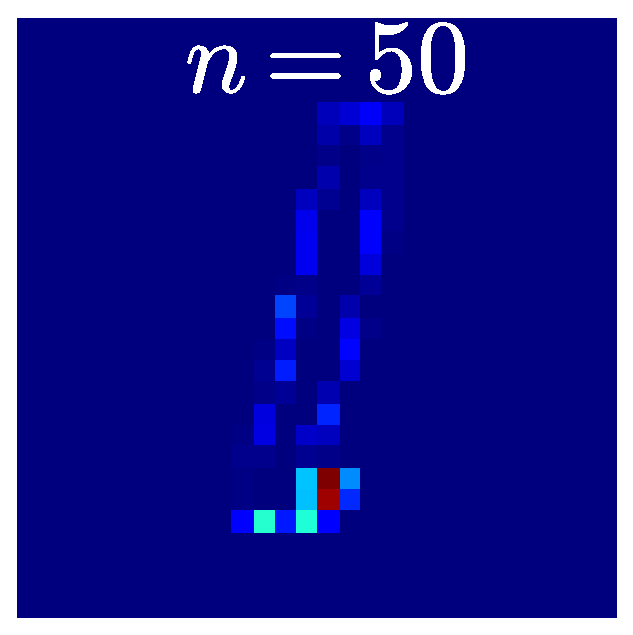
\includegraphics[width=0.1\linewidth]{figures/pixel_relevance_50.eps}
		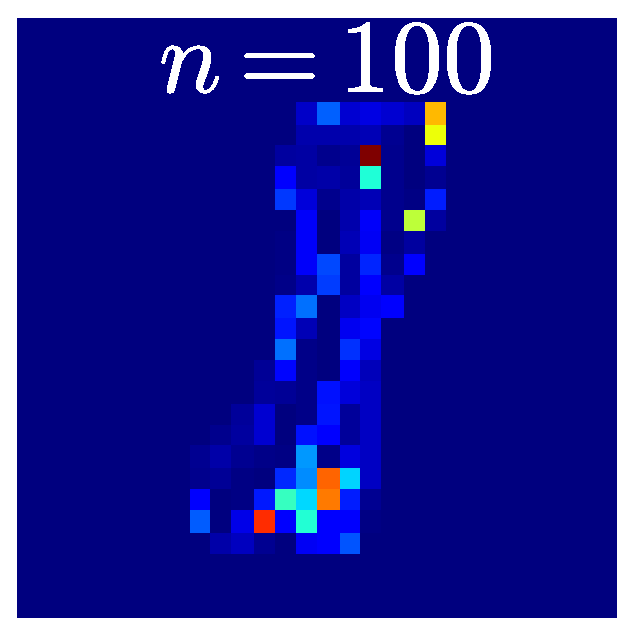
\includegraphics[width=0.1\linewidth]{figures/pixel_relevance_100.eps}
		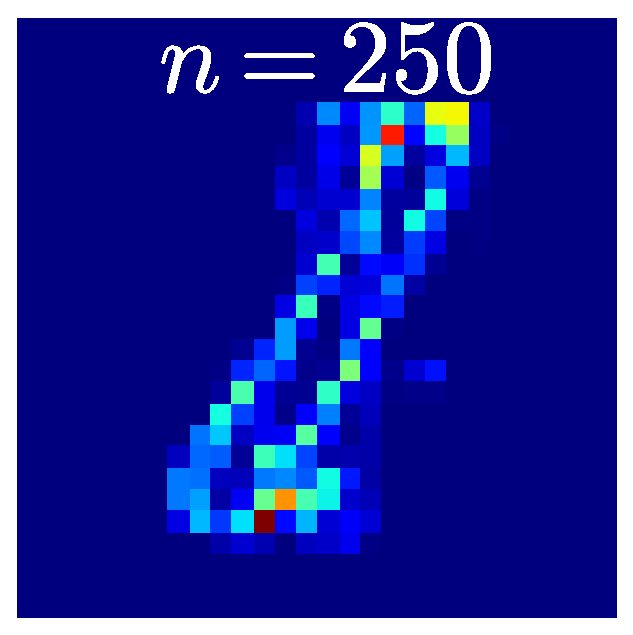
\includegraphics[width=0.1\linewidth]{figures/pixel_relevance_250.eps}
		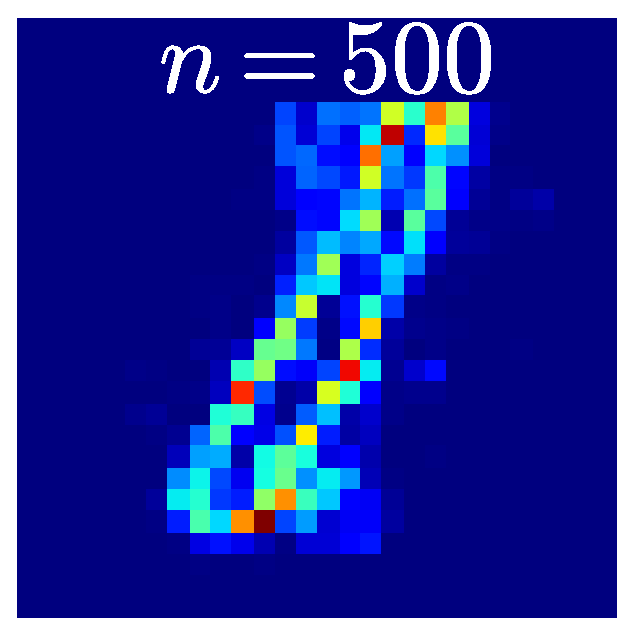
\includegraphics[width=0.1\linewidth]{figures/pixel_relevance_500.eps}
		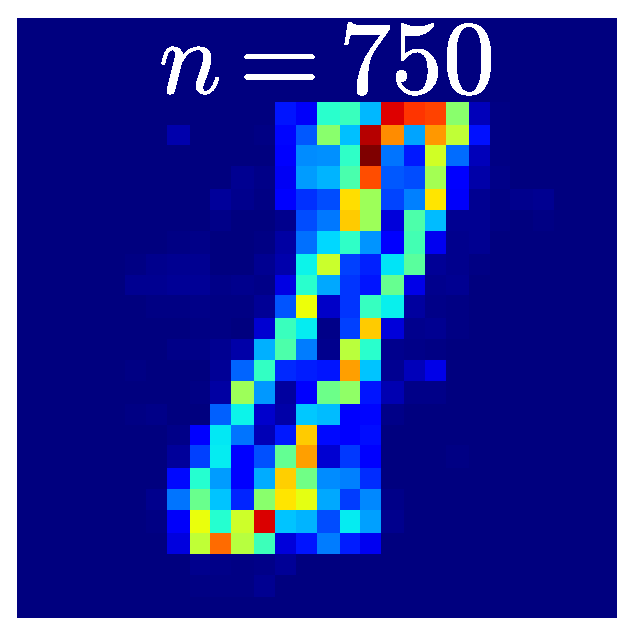
\includegraphics[width=0.1\linewidth]{figures/pixel_relevance_750.eps}
		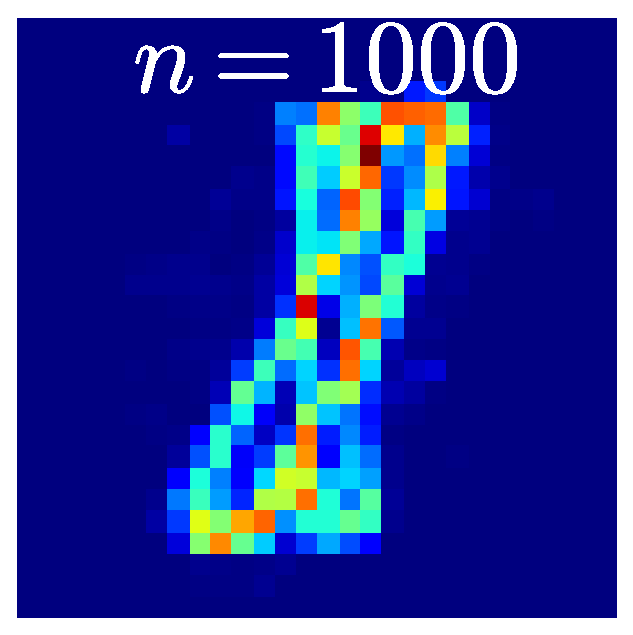
\includegraphics[width=0.1\linewidth]{figures/pixel_relevance_1000.eps}
		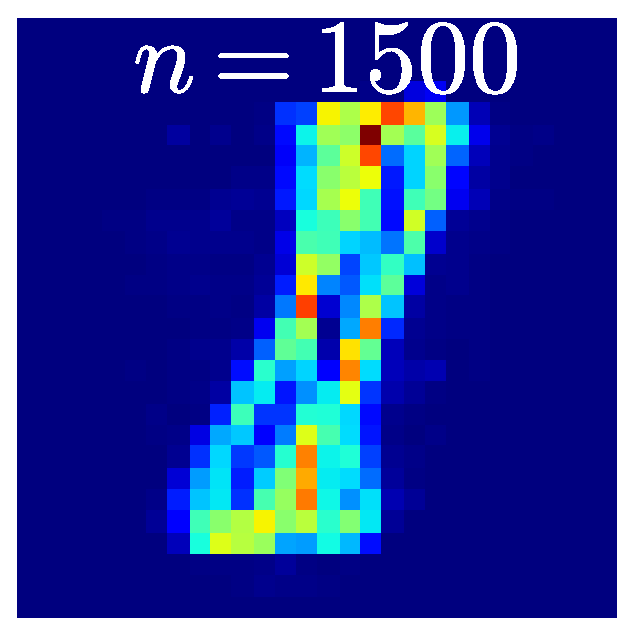
\includegraphics[width=0.1\linewidth]{figures/pixel_relevance_1500.eps}
		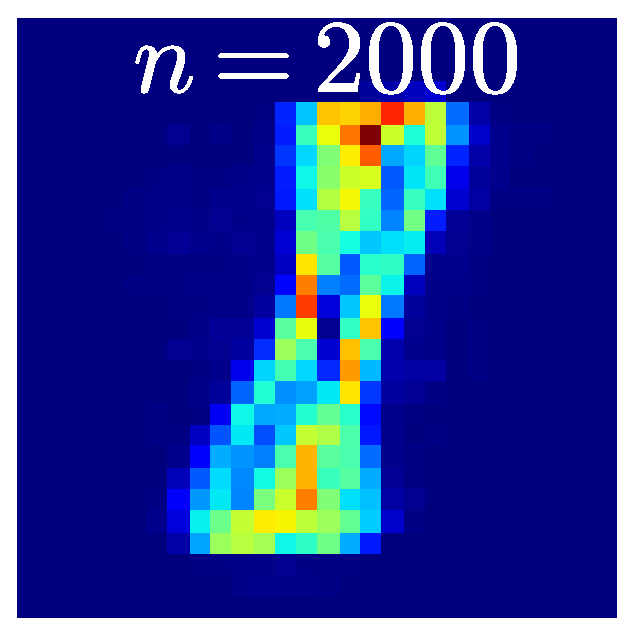
\includegraphics[width=0.1\linewidth]{figures/pixel_relevance_2000.eps}
		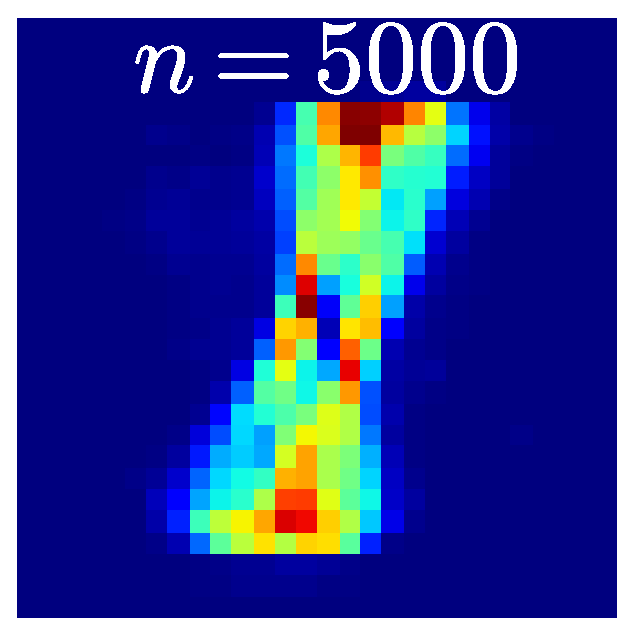
\includegraphics[width=0.1\linewidth]{figures/pixel_relevance_5000.eps}
		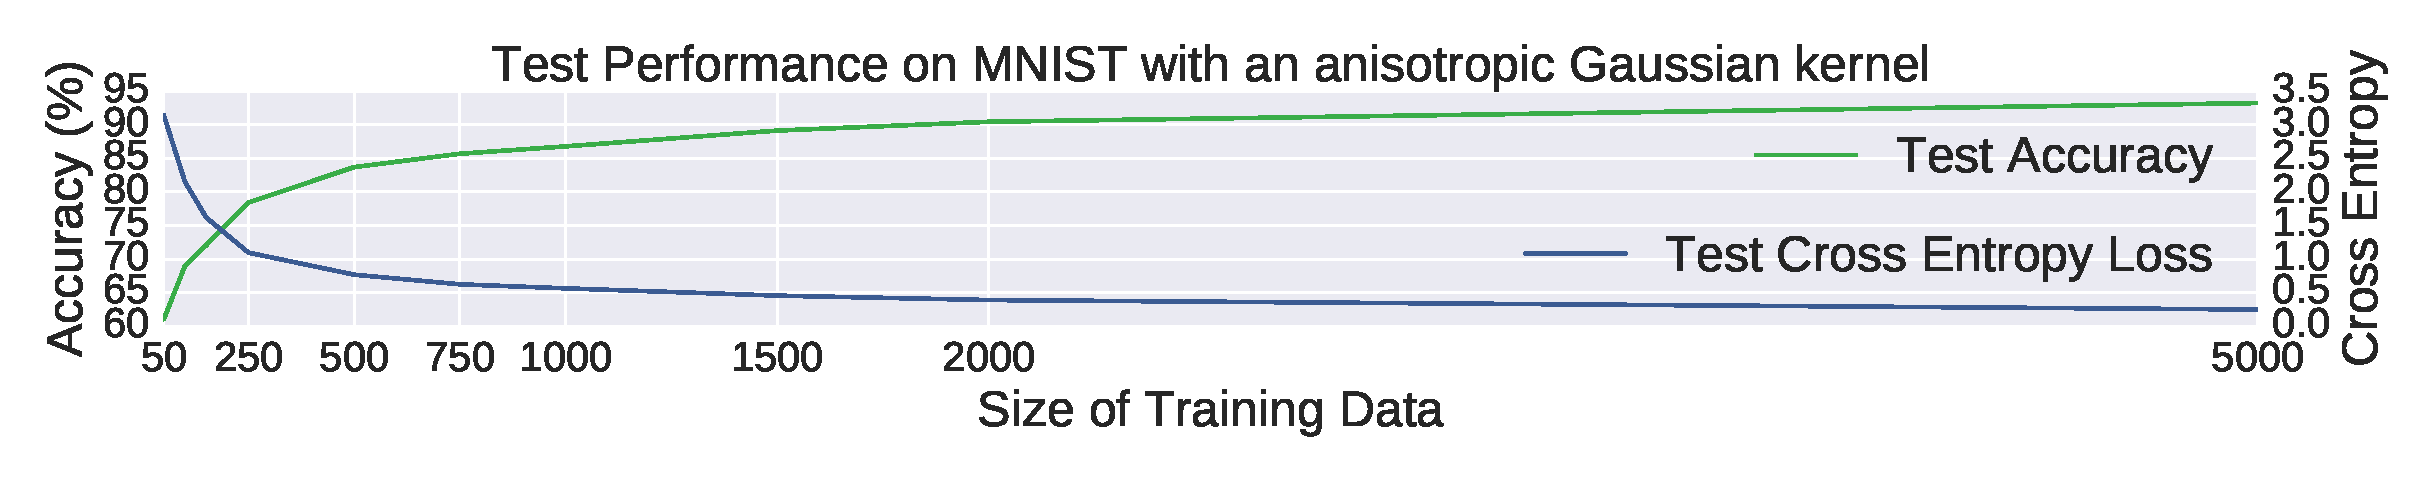
\includegraphics[width=\linewidth]{figures/test_performance.eps}
		\caption{Training the kernel embedding classifier on the MNIST digits dataset with an anisotropic Gaussian kernel. Top: Learned length scales for each pixel; Bottom: Performance on the test set.}
		\label{fig:pixel_relevance}
	\end{figure}
		
\section{Conclusion}

	\note{Summarise main contribution. Specifically, the guaranteed convergence of the kernel embedding classifier in both decision probability and information entropy, the Rademacher complexity based hyperparameter training scheme, the stochastic gradient descent version thereof which allows scalable training, the application of such flexible training methods to train deep convolutional features, and the fully probabilistic inference on both inputs and outputs. Focus the point of the paper as that this is a new and elegant formulation of a fully probabilistic classifier (not just in the outputs, but even in the inputs) with complexity bound based training. Being formulated as type of kernel conditional embedding learning, all the nice properties from the Hilbert space embedding world can be imported into this framework. In practice, even though the mathematical theory of kernel embeddings can be tricky, the resulting algorithms are very elegant and simple, so that implementation is quick and easy. Being very general, there should be a lot of things we can do in the future to improve it or build upon it.}
	
	\textbf{Future Work}: \note{(Not that polished)}
	
	\begin{itemize}
		\item \textbf{Hyperparameter Training through Local Rademacher Complexity.} In parallel with the work of \cite{xu2016local}, we can derive an upper bound for the \textit{local Rademacher complexity} of our kernel embedding classifier. In contrast to the global Rademacher complexity, the local Rademacher complexity of a model produces a sharper generalization error bound and a faster convergence rate. Specifically, for our classifier, it is upper bounded by the tail sum of the sorted eigenvalues of $B^{T} (K + n \lambda I)^{-1} K (K + n \lambda I)^{-1} B$. The complication is that there is an extra design choice to be made: from which eigenvalue should the tail sum start. Preliminary experiments that we have done so far shows that this choice affects the training a lot, and thus more work is needed to theorise how this choice should be done, and if it really improves classification performance consistently at the end of the day.

		\item \textbf{Multiple Kernel Learning and Shallow-Deep Kernels.} With kernel methods, newer and more flexible kernel classes can always be formed by convex combinations of simpler positive definite kernels. We can explore kernel and hyperparameter learning for these architectures under the kernel embedding classification framework that we developed in this paper.
		
		\textbf{Multiple Kernel Learning}. In summary, multiple kernel learning is traditionally interested in forming a new kernel $k(x, x') := \sum_{i = 1}^{p} \alpha_{i} k_{i}(x, x')$ from simpler kernels $k_{i}(x, x')$ by finding the optimal coefficient vector $\{\alpha_{i}\}_{i = 1}^{p}$ with respect to its learning task under convexity constraints. While this convex optimisation problem is quite tractable, each kernel component $k_{i}$ stays fixed, so that it is up to the practitioners to choose and tune each kernel component a-priori. With the kernel embedding classification framework, hyperparameter training is very general, and makes no restrictions on where the trainable parameters must appear (with the trade-off being that the optimisation may become non-convex). As such, we can construct newer kernels through $k(x, x'; \theta) := \sum_{i = 1}^{p} \alpha_{i} k_{i}(x, x'; \theta_{i})$ and generalise the multiple kernel learning problem to one that finds the optimal coefficient vector $\{\alpha_{i}\}_{i = 1}^{p}$ and kernel parameters $\{\theta_{i}\}_{i = 1}^{p}$. Of course, the regularisation parameter $\lambda$ is jointly learned at the same time.
		
		\textbf{Shallow-Deep Kernels}. Similarly, another way of convexly combining kernels is through a simple tensor multiplication, $k([x, z]^{T}, [x', z']^{T}; \theta_{\mathcal{X}}, \theta_{\mathcal{Z}}) := k_{\mathcal{X}}(x, x'; \theta_{\mathcal{X}}) k_{\mathcal{Z}}(z, z'; \theta_{\mathcal{Z}})$. In this scenario, we can let $x \in \mathcal{X}$ to be the original unaltered example inputs, while $z = f(x; w) \in \mathcal{Z}$ be the output of the last hidden layer of a neural network, where we use $w$ to collectively denote all the weight and bias parameters of the neural network. In this way, $k_{\mathcal{X}}$ is a shallow kernel allowing a direct connection from input to output, while $k_{\mathcal{Z}}$ is a deep kernel performing multiple layers of feature extraction from the input before it is connected to the output. Again, because hyperparameter training is very general in the kernel embedding classification framework, it should be possible to jointly learn the kernel hyperparameters $\theta_{\mathcal{X}}, \theta_{\mathcal{Z}}$, the neural network weights and biases $w$, and the regularisation parameter $\lambda$.
		
		\item \textbf{Connection to other kernel models.} It should not be too surprising if we can find many connections or even equivalences to other kernel techniques. For example, if we look at the form of our decision probability estimator, it is also the same as the mean prediction of a Gaussian process regression, except we replace the real-valued targets in the regression case with the one-hot encoded class targets for our classification task. Of course, the main difference thereafter is how we train the two models. We turned to complexity based training partly because, unlike a Gaussian process, it is very difficult to find the marginal likelihood for a kernel embedding, and this has worked out well. However, future work can look into the direction of actually finding a way to compute or approximate the marginal likelihood for the kernel embedding classifier, making the link between Gaussian processes and kernel embeddings even stronger.
		
		Another simpler connection may be the k-nearest-neighbour classifier. For any stationary and radially symmetric kernel like the Gaussian and Matern kernels, shorter length scales usually produces a nearest-neighbour effect on the inference of kernel embedding classifiers. Of course, this is suboptimal, and the complexity based training developed in this paper would know better to not learn such a length scale. However, this link would illustrate the purpose and effectiveness of a complexity based training scheme for kernel methods.
		
		\item \textbf{Sampling and Generative Models.} While the kernel embedding classifier is trained as a discriminative model, at its core it is simply just a condition embedding of $\mathbb{P}_{Y | X}$. As such, we can do full probabilistic inference entirely in reproducing kernel Hilbert spaces and obtain the Hilbert space embeddings of $\mathbb{P}_{X | Y}$, similar to what we have touched upon in \cref{sec:mode_reconstruction}, or even simply of the marginals $\mathbb{P}_{X}$ and $\mathbb{P}_{Y}$. If we can recover these distributions as densities ($\mathbb{P}_{Y}$ would correspond to a probability mass function over a finite and discrete space $\mathbb{N}_{m}$ which is identical to the mean embedding already, and so this step would be trivial for $\mathbb{P}_{Y}$), then we would be able to model our data in a fully generative manner. In fact, in \cref{sec:mode_reconstruction} we have have already done so indirectly through reversing the embedding. Of course, this would require us to solve the pre-image problem of kernel embeddings, for which no general methodology exists yet besides a few heuristics with various assumptions. Nevertheless, assuming we can recover the densities well enough, we can then generate samples from those distributions. Alternatively, if we can instead sample from those distributions \textit{without} finding the pre-image, but by directly using the mean embeddings instead, that would make the kernel embedding classifier very useful as a generative modelling tool.
		
		\item \textbf{Target Label Kernel.} In this paper, we proposed to place a Kronecker delta kernel $l = \delta$ over the label space $\mathcal{Y} = \mathbb{N}_{m}$ as it is the simplest kernel over a discrete and finite domain. However, it is possible to place other kernels over the label space. A simple kernel is to have a `generalised Kronecker delta kernel' that has unit similarity when labels are the same, but a small, positive yet non-zero similarity when labels are different. If we set these cross similarity to be the same across all non-identical pairs of labels, then it is straight forward to show that the inference algorithm we developed in this paper stays the same. However, if we allow them to vary amongst each other as kernel parameters (between the range $(0, 1)$, in order to stay positive definite), then we suspect that these cross similarity coefficients would act as correlation factors between classes. The training algorithm we developed here does not prevent the target label kernel to have its own hyperparameters. As such, we should be able to learn the correlation effects between the classes effectively using the same training scheme. We suspect that this would make the empirical decision probabilities converge to a valid probability distribution faster. However, we also suspect that the training may become even more non-convex and optimisation to become more difficult.
		
		These factors may even give rise to new interpretable insights in terms of how different classes may be more related to each other. For example, in an image recognition task of animals, it may learn that, the class `horse' and 'pony' are much more similar than `horse' and `elephant' from the input features, and start to use the output correlations to focus on inferring about them as a group instead.
		\end{itemize}
	
\small
\bibliographystyle{apalike}
\bibliography{kernel_embedding}

\newpage
\appendix

\section{Information Entropy}
\label{sec:information_entropy}

	The kernel embedding classifier provides decision probabilities instead of just a single label prediction. Such a probabilistic classifier allows us to quantify the uncertainty of its predictions for any given example $x \in \mathcal{X}$ through the information entropy \citep{shannon1951prediction, jaynes1957information}. This is ideal for detecting the decision boundaries of the classifier and areas of low data density.
	
	We present two main approaches for inferring the information entropy from the classifier. Specifically, we would like to infer estimates for $h(x) := \mathbb{H}[Y | X = x] = - \sum_{c = 1}^{m} p_{c}(x) \log{p_{c}(x)} $, the information entropy of the possible labels $Y$ for a given example $X = x$.
	
	The first approach is straight forward, which involves simply computing the information entropy with the clip normalised probabilities \eqref{eq:probability_clip_normalise}, at the query point $x \in \mathcal{X}$,
	\begin{equation}
		\tilde{h}(x) := - \sum_{c = 1}^{m} \tilde{p}_{c}(x) \log{\tilde{p}_{c}(x)}.
	\label{eq:entropy_clip_normalise}
	\end{equation}
	We call \eqref{eq:entropy_clip_normalise} the \textit{clip-normalised information entropy}. Since $\tilde{p}_{c}(x)$ converges pointwise to $p_{c}(x)$ with increasing data, $\tilde{h}(x)$ also converges pointwise to $h(x)$.
	
	Just as decision probabilities can be expressed as an expectation of indicator functions, information entropy can be expressed as expected information \footnote{Note that while $\mathbb{P}[Y = c | X = x]$ is a constant, we employ the shorthand notation $\mathbb{P}[Y| X = x]$ for the random variable $g(Y)$ where $g(y) := \mathbb{P}[Y = y | X = x]$.},
	\begin{equation}
	\begin{aligned}
		\mathbb{H}[Y | X = x] &= - \sum_{c = 1}^{m} \mathbb{P}[Y = c| X = x] \log{\mathbb{P}[Y = c | X = x]} \\
		&= \mathbb{E}[- \log{\mathbb{P}[Y | X = x]} | X = x] \\
		&= \mathbb{E}[u_{x}(Y) | X = x],
	\end{aligned}
	\end{equation}
	where $u_{x}(y) := - \log{\mathbb{P}[Y = y | X = x]}$ is the \textit{information} (in nats) we would gain when we discover that example $x$ actually has label $y$. If $u_{x} : \mathbb{N}_{m} \to \mathbb{R}$ is in the RKHS $\mathcal{H}_{\delta}$, then we know that this expectation can also be approximated by $\langle \hat{\mu}_{Y | X = x}, u_{x} \rangle$. This is the basis of our second approach.
	
	Assuming that $\mathbb{P}[Y = y | X = x]$ is never exactly zero for all labels $y \in \mathcal{Y}$ and examples $x \in \mathcal{X}$, then $u_{x}(y)$ is bounded on its discrete domain $\mathbb{N}_{m}$. We can thus write $u_{x} = \sum_{c = 1}^{m} - \log{\mathbb{P}[Y = c | X = x]} \delta(c, \cdot)$ which shows that $u_{x}$ is in the span of the canonical kernel features and is thus in the RKHS. Hence, similar to the case with decision probabilities, with $u_{x} \in \mathcal{H}_{\delta}$ and $\bvec{u}_{x} := \{u_{x}(y_{i})\}_{i = 1}^{n}$ we let $g = u_{x}$ in \eqref{eq:empirical_conditional_expectation} and estimate $h(x)$ by
	\begin{equation}
		\langle \hat{\mu}_{Y | X = x}, u_{x} \rangle = \bvec{u}_{x}^{T} (K + n \lambda I)^{-1} \bvec{k}_{x}.
	\end{equation}
	Unfortunately, $u_{x}$ is not known exactly, since $\mathbb{P}[Y = y | X = x]$ is not known exactly. Instead, since $\hat{p}_{c}(x)$ is a consistent estimate for $\mathbb{P}[Y = c | X = x]$ by \cref{thm:probability_convergence}, we propose to replace $u_{x}(y)$ with the negative log of $\hat{p}_{y}(x)$. However, we cannot simply take the log of this estimator, as $\hat{p}_{y}(x)$ may produce non-positive estimates to the prediction probabilities. The straight forward way to mitigate this problem is to clip $\hat{p}_{y}(x)$ from the bottom by a very small number, before taking the log. However, experiments show that this produces non-smooth estimates over $\mathcal{X}$ and the degree of smoothness varies drastically between different choices of that small number (see \cref{app:design_choices}). Instead, in virtue of the fact that $\lim_{p \to 0} - p \log{p} = 0$ even though $\lim_{p \to 0} - \log{p} = \infty$, we simply define the information estimate $\hat{u}_{x}(y)$ as zero if the empirical decision probability is non-positive,
	\begin{equation}
		\hat{u}_{x}(y) := \begin{cases}
		- \log{\hat{p}_{y}(x)} & \mathrm{if } \quad \hat{p}_{y}(x) > 0 \\
		0 & \mathrm{otherwise}. \end{cases}
	\label{eq:empirical_information}
	\end{equation}
	It remains to show that $\hat{u}_{x} \in \mathcal{H}_{\delta}$. Indeed, the identity $\hat{u}_{x} = \sum_{c = 1}^{m} \hat{u}_{x}(c) \delta(c, \cdot)$ holds and thus $\hat{u}_{x}$ is in the span of the kernel canonical features. We then arrive at the following estimate for $h(x)$,
	\begin{equation}
		\hat{h}(x) := \langle \hat{\mu}_{Y | X = x}, \hat{u}_{x} \rangle = \hat{\bvec{u}}_{x}^{T} (K + n \lambda I)^{-1} \bvec{k}_{x},
		\label{eq:empirical_information_entropy}
	\end{equation}
	where $\hat{\bvec{u}}_{x} := \{\hat{u}_{x}(y_{i})\}_{i = 1}^{n}$. Similar to the case with decision probabilities \eqref{eq:decision_probability}, the information entropy estimate \eqref{eq:empirical_information_entropy} is not guaranteed to be non-negative. However, in practice these negative values are close to zero. Furthermore, negative estimated information entropy implies that the model is very confident about its prediction, and it suffices to simply clip the entropy at zero if strict information entropy is required (see \cref{app:design_choices}). We give the proof of convergence of \eqref{eq:empirical_information_entropy} in \cref{app:convergence_theorems}.
	\begin{theorem}[Uniform Convergence of Empirical Information Entropy Function]
		\label{thm:entropy_convergence_copy}
		Assuming that $k(x, \cdot)$ is in the image of $C_{XX}$, the empirical information entropy function $\hat{h} : \mathcal{X} \to \mathbb{R}$ \eqref{eq:empirical_information_entropy} converges uniformly to the true information entropy function $h : \mathcal{X} \to [0, \infty)$ at a stochastic rate of at least $O_{p}((n \lambda)^{-\frac{1}{2}} + \lambda^{\frac{1}{2}})$.
	\end{theorem}
	
\section{Convergence Theorems}
\label{app:convergence_theorems}

	In this section we provide a few theorems, lemmas, and derivations which proves the convergence properties of estimators derived from our kernel embedding classifier.
	
	We consider the case in which a dataset, represented by the collection of random variables $\{X_{i}, Y_{i}\}_{i = 1}^{n}$ where $X_{i} : \Omega \to \mathcal{X}$,  $Y_{i} : \Omega \to \mathcal{Y}$ for all $i \in \mathbb{N}_{n}$, is collected in a \textit{iid} fashion from some distribution $\mathbb{P}_{X Y}$. That is $\{X_{i}, Y_{i}\} \sim \mathbb{P}_{X Y}$ for all $i \in \mathbb{N}_{n}$ and each observed sample is independent from each other. Suppose we have an estimator function $\hat{f}^{(n)} : \mathcal{X} \to \mathbb{R}$ which is to estimate some target function  $f : \mathcal{X} \to \mathbb{R}$, usually but not necessarily derived from $\mathbb{P}_{Y |X }$, empirically using the collected dataset $\{X_{i}, Y_{i}\}_{i = 1}^{n}$ of size $n \in \mathbb{N}_{+}$. Here, we use the superscript $(n)$ to denote the estimator's dependence on the dataset. From this point on, we drop this superscript to avoid cluttered notation. However, one should keep in mind that $\hat{f}$ is estimated using the dataset $\{X_{i}, Y_{i}\}_{i = 1}^{n}$ and is thus random over the possible data observation events $\omega \in \Omega$. We would like to provide a sense of the stochastic convergence of $\hat{f}$ to $f$ by providing an upper bound of their absolute pointwise difference $| \hat{f}(x) - f(x) |$ which we know convergences to zero at some stochastic rate. Since the kernel embedding classifier is based on conditional embeddings, this upper bound will be provided by the RKHS norm of the error between empirical and true conditional embeddings. Specifically, the empirical conditional embedding stochastically converges to the true conditional embedding $\mu_{Y | X = x}$ in the RKHS norm at a rate of $O_{p}((n \lambda)^{-\frac{1}{2}} + \lambda^{\frac{1}{2}})$, under the assumption that $k(x, \cdot)$ is in the image of $C_{XX}$ \citet[Theorem 6]{song2009hilbert}. That is,
	
		\begin{equation}
			\forall x \in \mathcal{X}, \; \epsilon > 0, \; \exists M_{\epsilon} > 0 \quad s.t. \quad \mathbb{P}\Big[\big\| \hat{\mu}_{Y | X = x} - \mu_{Y | X = x} \big\|_{\mathcal{H}_{l}} > M_{\epsilon} \Big((n \lambda)^{-\frac{1}{2}} + \lambda^{\frac{1}{2}}\Big)\Big] < \epsilon.
		\label{eq:empirical_conditional_embedding_stochastic_convergence}
		\end{equation}
	
	\begin{theorem}[Pointwise and Uniform Convergence of Estimators based on Conditional Embeddings]
		\label{thm:pointwise_uniform_convergence}
		Suppose that $k(x, \cdot)$ is in the image of $C_{XX}$ and that there exists $0 \leq \gamma(x) < \infty$ such that for some estimator function $\hat{f} : \mathcal{X} \to \mathbb{R}$ and target function  $f : \mathcal{X} \to \mathbb{R}$,
		
		\begin{equation}
			| \hat{f}(x) - f(x) | \leq \gamma(x) \big\| \hat{\mu}_{Y | X = x} - \mu_{Y | X = x} \big\|_{\mathcal{H}_{l}}, \forall x \in \mathcal{X},
		\label{eq:estimator_error_bound}
		\end{equation}
		 
		then the estimator $\hat{f}$ converges pointwise to the target $f$ at a stochastic rate of at least $O_{p}((n \lambda)^{-\frac{1}{2}} + \lambda^{\frac{1}{2}})$. Further, if $\gamma(x) = \gamma$ is independent of $x \in \mathcal{X}$, then this convergence is uniform.
		
		\begin{proof}
			
			Suppose that there exists $0 \leq \gamma(x) < \infty$ such that \eqref{eq:estimator_error_bound} is satisfied. Note that this statement holds for all possible datasets represented by the collection of random variables $\{X_{i}, Y_{i}\}_{i = 1}^{n}$ where $X_{i} : \Omega \to \mathcal{X}$,  $Y_{i} : \Omega \to \mathcal{Y}$ for all $i \in \mathbb{N}_{n}$. Thus, for any constant $C$, the implication statement $\big\| \hat{\mu}_{Y | X = x} - \mu_{Y | X = x} \big\|_{\mathcal{H}_{\delta}} \leq C \implies | \hat{f}(x) - f(x) | \leq C \gamma(x)$ holds for all possible data observation events $\omega \in \Omega$. Writing this explicitly in event space translates this to a probability statement,
			
			\begin{equation}
			\begin{aligned}
				\{\omega \in \Omega : \big\| \hat{\mu}_{Y | X = x} - \mu_{Y | X = x} \big\|_{\mathcal{H}_{l}} \leq C\} &\subseteq \{\omega \in \Omega : | \hat{f}(x) - f(x) | \leq C \gamma(x)\} \\
				\implies \mathbb{P}\Big[\big\| \hat{\mu}_{Y | X = x} - \mu_{Y | X = x} \big\|_{\mathcal{H}_{l}} \leq C\Big] &\leq \mathbb{P}\Big[| \hat{f}(x) - f(x) | \leq C \gamma(x) \Big].
			\label{eq:probability_statement}
			\end{aligned}
			\end{equation}
			
			Since we assume that $k(x, \cdot) \in \mathrm{image}(C_{XX})$, statement \eqref{eq:empirical_conditional_embedding_stochastic_convergence} is valid. By letting $C = M_{\epsilon} ((n \lambda)^{-\frac{1}{2}} + \lambda^{\frac{1}{2}})$ in \eqref{eq:probability_statement}, we immediately have that the probability inequality in statement \eqref{eq:empirical_conditional_embedding_stochastic_convergence} is also true if we replace $\| \hat{\mu}_{Y | X = x} - \mu_{Y | X = x} \|$ with $| \hat{f}(x) - f(x) |$ and $M_{\epsilon}$ with $\gamma(x) M_{\epsilon}$,
			
			\begin{equation}
			\begin{aligned}
			\mathbb{P}\Big[\big\| \hat{\mu}_{Y | X = x} - \mu_{Y | X = x} \big\|_{\mathcal{H}_{l}} > M_{\epsilon} \Big((n \lambda)^{-\frac{1}{2}} + \lambda^{\frac{1}{2}}\Big)\Big] &< \epsilon \\
			\implies 1 - \mathbb{P}\Big[\big\| \hat{\mu}_{Y | X = x} - \mu_{Y | X = x} \big\|_{\mathcal{H}_{l}} \leq M_{\epsilon} \Big((n \lambda)^{-\frac{1}{2}} + \lambda^{\frac{1}{2}}\Big)\Big] &< \epsilon \\
			\implies \mathbb{P}\Big[\big\| \hat{\mu}_{Y | X = x} - \mu_{Y | X = x} \big\|_{\mathcal{H}_{l}} \leq M_{\epsilon} \Big((n \lambda)^{-\frac{1}{2}} + \lambda^{\frac{1}{2}}\Big)\Big] &> 1 -  \epsilon \\
			\implies \mathbb{P}\Big[| \hat{f}(x) - f(x) | \leq \gamma(x) M_{\epsilon} \Big((n \lambda)^{-\frac{1}{2}} + \lambda^{\frac{1}{2}}\Big)\Big] &> 1 -  \epsilon \\
			\implies 1 - \mathbb{P}\Big[| \hat{f}(x) - f(x) | \leq \gamma(x) M_{\epsilon} \Big((n \lambda)^{-\frac{1}{2}} + \lambda^{\frac{1}{2}}\Big)\Big] &< \epsilon \\
			\implies \mathbb{P}\Big[| \hat{f}(x) - f(x) | > \gamma(x) M_{\epsilon} \Big((n \lambda)^{-\frac{1}{2}} + \lambda^{\frac{1}{2}}\Big)\Big] &< \epsilon.
			\end{aligned}	
			\end{equation}
			
			where we employed statement \eqref{eq:probability_statement} between the third and fourth line for $C = M_{\epsilon} ((n \lambda)^{-\frac{1}{2}} + \lambda^{\frac{1}{2}})$. Therefore, since $M_{\epsilon}$ is arbitrary, define $\tilde{M}_{\epsilon}(x) := \gamma(x) M_{\epsilon}$ so that, with the above result, the statement \eqref{eq:empirical_conditional_embedding_stochastic_convergence} implies the following,

			\begin{equation}
				\forall x \in \mathcal{X}, \; \epsilon > 0, \; \exists \tilde{M}_{\epsilon}(x) > 0 \quad s.t. \quad \mathbb{P}\Big[\big| \hat{f}(x) - f(x) \big| > \tilde{M}_{\epsilon}(x) \Big((n \lambda)^{-\frac{1}{2}} + \lambda^{\frac{1}{2}}\Big)\Big] < \epsilon.
			\end{equation}
	
			In other words, the function $\hat{f}$ stochastically converges pointwise to $f$ with a rate of at least $O_{p}((n \lambda)^{-\frac{1}{2}} + \lambda^{\frac{1}{2}})$. The convergence is pointwise as the constant $\tilde{M}_{\epsilon}(x)$ may be different for each point $x \in \mathcal{X}$. If $\gamma(x) = \gamma$ such that $\tilde{M}_{\epsilon}(x) = \tilde{M}_{\epsilon}$ does not depend on $x \in \mathcal{X}$, then this stochastic convergence is uniform in its domain $\mathcal{X}$.
		\end{proof}
		
	\end{theorem}
	
	With \cref{thm:pointwise_uniform_convergence}, we can now show the convergence of various estimators based on the conditional embedding, as long as we can show that their estimator error is upper bounded by a multiple of the conditional embedding error in the RKHS norm. As such, we turn to the convergence of the empirical decision probability function \eqref{eq:empirical_decision_probability} below.

	\begin{theorem}[Uniform Convergence of Empirical Decision Probability Function]
		\label{thm:probability_convergence}
		Assuming that $k(x, \cdot)$ is in the image of $C_{XX}$, the empirical decision probability function $\hat{p}_{c} : \mathcal{X} \to \mathbb{R}$ \eqref{eq:empirical_decision_probability} converges uniformly to the true decision probability $p_{c} : \mathcal{X} \to [0, 1]$ \eqref{eq:decision_probability} at a stochastic rate of at least $O_{p}((n \lambda)^{-\frac{1}{2}} + \lambda^{\frac{1}{2}})$ for all $c \in \mathcal{Y} = \mathbb{N}_{m}$.
		
		\begin{proof}
			Consider the pointwise absolute difference between the decision probability and its empirical estimate,
			
			\begin{equation}
			\begin{aligned}
				| \hat{p}_{c}(x) - p_{c}(x) | &= | \langle \hat{\mu}_{Y | X = x}, \mathbb{1}_{c} \rangle - \langle \mu_{Y | X = x}, \mathbb{1}_{c} \rangle | \\
				&= | \langle \hat{\mu}_{Y | X = x} - \mu_{Y | X = x}, \mathbb{1}_{c} \rangle | \\
				&\leq \big\| \hat{\mu}_{Y | X = x} - \mu_{Y | X = x} \big\|_{\mathcal{H}_{\delta}} \big\| \mathbb{1}_{c} \big\|_{\mathcal{H}_{\delta}},
			\label{eq:decision_probability_error_upper_bound}
			\end{aligned}
			\end{equation}
			
			where the last inequality follows from the Cauchy–Schwarz inequality in a Hilbert space.
			
			From \eqref{eq:indicator_function}, since $\mathbb{1}_{c} = \delta(c, \cdot)$ and using the fact that $\delta$ is a reproducing kernel, we have that for all $c \in \mathcal{Y} = \mathbb{N}_{m}$.
			
			\begin{equation}
			\begin{aligned}
				\big\| \mathbb{1}_{c} \big\|_{\mathcal{H}_{\delta}}^{2} = \langle \mathbb{1}_{c}, \mathbb{1}_{c} \rangle = \langle \delta(c, \cdot), \delta(c, \cdot) \rangle = \delta(c, c) = 1.
			\label{eq:indicator_rkhs_norm}
			\end{aligned}
			\end{equation}
			
			Therefore, by \cref{thm:pointwise_uniform_convergence} with $\gamma(x) = 1$ independent of $x \in \mathcal{X}$, $\hat{p}_{c}$ converges uniformly to $p_{c}$ at a stochastic rate of at least $O_{p}((n \lambda)^{-\frac{1}{2}} + \lambda^{\frac{1}{2}})$ for all $c \in \mathcal{Y} = \mathbb{N}_{m}$.
			
			%		Consequently, $| \hat{p}_{c}(x) - p_{c}(x) | \leq \big\| \hat{\mu}_{Y | X = x}^{(n)} - \mu_{Y | X = x} \big\|_{\mathcal{H}_{\delta}}$ for all $x \in \mathcal{X}$, where the right hand side of which approaches zero stochastically at rate $O_{p}((n \lambda)^{-\frac{1}{2}} + \lambda^{\frac{1}{2}})$ since we assume that $k(x, \cdot) \in \mathrm{image}(C_{XX})$, so that $\hat{p}_{c}$ converges pointwise to $p_{c}$ at least at this rate. The convergence rate does not depend on $x \in \mathcal{X}$, so this (stochastic) convergence is pointwise uniform.
			
%			Consequently, for all $x \in \mathcal{X}$ and $c \in \mathcal{Y}$, we have 
%			
%			\begin{equation}
%				| \hat{p}_{c}(x) - p_{c}(x) | \leq \big\| \hat{\mu}_{Y | X = x} - \mu_{Y | X = x} \big\|_{\mathcal{H}_{\delta}}.
%			\label{eq:uniform_convergence}
%			\end{equation}
%			
%			This is true for all possible datasets represented by the collection of random variables $\{X_{i}, Y_{i}\}_{i = 1}^{n}$ where $X_{i} : \Omega \to \mathcal{X}$,  $Y_{i} : \Omega \to \mathcal{Y}$ for all $i \in \mathbb{N}_{n}$. Thus, for any constant $C$, the implication statement $\big\| \hat{\mu}_{Y | X = x} - \mu_{Y | X = x} \big\|_{\mathcal{H}_{\delta}} \leq C \implies | \hat{p}_{c}(x) - p_{c}(x) | \leq C$ holds for all possible data observation events $\omega \in \Omega$. Writing this explicitly in event space translates this to a probability statement,
%			
%			\begin{equation}
%			\begin{aligned}
%			\{\omega \in \Omega : \big\| \hat{\mu}_{Y | X = x} - \mu_{Y | X = x} \big\|_{\mathcal{H}_{\delta}} \leq C\} &\subseteq \{\omega \in \Omega : | \hat{p}_{c}(x) - p_{c}(x) | \leq C\} \\
%			\implies \mathbb{P}\Big[\big\| \hat{\mu}_{Y | X = x} - \mu_{Y | X = x} \big\|_{\mathcal{H}_{\delta}} \leq C\Big] &\leq \mathbb{P}\Big[| \hat{p}_{c}(x) - p_{c}(x) | \leq C \Big].
%			\label{eq:probability_statement}
%			\end{aligned}
%			\end{equation}
%			
%			Since we assume that $k(x, \cdot) \in \mathrm{image}(C_{XX})$, statement \eqref{eq:empirical_conditional_embedding_stochastic_convergence} is valid. By letting $C = M_{\epsilon} ((n \lambda)^{-\frac{1}{2}} + \lambda^{\frac{1}{2}})$ in \eqref{eq:probability_statement}, we immediately have that the probability inequality in statement \eqref{eq:probability_statement} is also true if we replace $\| \hat{\mu}_{Y | X = x} - \mu_{Y | X = x} \|$ with $| \hat{p}_{c}(x) - p_{c}(x) |$, % the RKHS norm between the empirical and true embeddings to the absolute difference between the empirical decision probability and the true decision probability,
%			
%			\begin{equation}
%			\begin{aligned}
%			\mathbb{P}\Big[\big\| \hat{\mu}_{Y | X = x} - \mu_{Y | X = x} \big\|_{\mathcal{H}_{l}} > M_{\epsilon} \Big((n \lambda)^{-\frac{1}{2}} + \lambda^{\frac{1}{2}}\Big)\Big] &< \epsilon \\
%			\implies 1 - \mathbb{P}\Big[\big\| \hat{\mu}_{Y | X = x} - \mu_{Y | X = x} \big\|_{\mathcal{H}_{l}} \leq M_{\epsilon} \Big((n \lambda)^{-\frac{1}{2}} + \lambda^{\frac{1}{2}}\Big)\Big] &< \epsilon \\
%			\implies \mathbb{P}\Big[\big\| \hat{\mu}_{Y | X = x} - \mu_{Y | X = x} \big\|_{\mathcal{H}_{l}} \leq M_{\epsilon} \Big((n \lambda)^{-\frac{1}{2}} + \lambda^{\frac{1}{2}}\Big)\Big] &> 1 -  \epsilon \\
%			\implies \mathbb{P}\Big[| \hat{p}_{c}(x) - p_{c}(x) | \leq M_{\epsilon} \Big((n \lambda)^{-\frac{1}{2}} + \lambda^{\frac{1}{2}}\Big)\Big] &> 1 -  \epsilon \\
%			\implies 1 - \mathbb{P}\Big[| \hat{p}_{c}(x) - p_{c}(x) | \leq M_{\epsilon} \Big((n \lambda)^{-\frac{1}{2}} + \lambda^{\frac{1}{2}}\Big)\Big] &< \epsilon \\
%			\implies \mathbb{P}\Big[| \hat{p}_{c}(x) - p_{c}(x) | > M_{\epsilon} \Big((n \lambda)^{-\frac{1}{2}} + \lambda^{\frac{1}{2}}\Big)\Big] &< \epsilon.
%			\end{aligned}	
%			\end{equation}
%			
%			In other words, the function $\hat{p}_{c}$ stochastically converges pointwise to $p_{c} := \mathbb{P}[Y = c | X = \cdot]$ with a rate of at least $O_{p}((n \lambda)^{-\frac{1}{2}} + \lambda^{\frac{1}{2}})$. The convergence rate does not depend on $x \in \mathcal{X}$ nor $c \in \mathbb{N}_{m}$, so this stochastic convergence is pointwise uniform in its domain $\mathcal{X}$ across all label classes.
			
		\end{proof}
	\end{theorem}
	
	The above proof is for uniform convergence over all $x \in \mathcal{X}$ at the stochastic rate of at least $O_{p}((n \lambda)^{-\frac{1}{2}} + \lambda^{\frac{1}{2}})$. Intuitively, however, for stationary zero-centred kernels like the Gaussian kernel, the convergence rate may be higher at regions of high data density, since the kernel effects, being centred around the training data, are stronger at these regions. The worse case convergence rate described here in the theorem would be a tight lower bound for regions in $\mathcal{X}$ with lower data density, where the kernel effects have decayed and most empirical probabilities are smaller and further from summing up to one.
	
	Because the label space $\mathcal{Y} = \mathbb{N}_{m}$ is discrete and finite, \textit{bounded} functions $g \in \mathcal{H}_{\delta}$ in the RKHS are actually equivalent to their vector representations $\bvec{g} := \{g(c)\}_{c = 1}^{m}$, because one can always write $g = \sum_{c = 1}^{m} g(c) \delta(c, \cdot)$. This immediately implies that inner products in this space are simply the usual dot products in a Euclidean space, since
	
	\begin{equation}
	\begin{aligned}
	\langle g_{1}, g_{2} \rangle_{\mathcal{H}_{\delta}} &= \bigg\langle \sum_{c = 1}^{m} g_{1}(c) \delta(c, \cdot), \sum_{c' = 1}^{m} g_{2}(c') \delta(c', \cdot)  \bigg\rangle_{\mathcal{H}_{\delta}} \\
	&= \sum_{c = 1}^{m} \sum_{c' = 1}^{m} g_{1}(c) g_{2}(c') \langle \delta(c, \cdot), \delta(c', \cdot) \rangle_{\mathcal{H}_{\delta}} \\
	&= \sum_{c = 1}^{m} g_{1}(c) g_{2}(c) \\
	&= \bvec{g}_{1} \cdot \bvec{g}_{2}.
	\end{aligned}
	\end{equation}
	
	Consequently, the RKHS norm for bounded functions $g \in \mathcal{H}_{\delta}$ is simply the $\ell_{2}$-norm of its vector representation $\bvec{g}$,
	
	\begin{equation}
	\lVert g \rVert_{\mathcal{H}_{\delta}} = \lVert \bvec{g} \rVert_{\ell_{2}}.
	\label{eq:rkhs_norm_is_l2_norm}
	\end{equation}

	A special and convenient result that arises due to this discrete and finite label space is that the decision probabilities and its empirical estimate are simply the conditional embeddings and its empirical estimate.
	
	\begin{claim}[Decision Probabilities are Conditional Embeddings]
	\label{thm:probability_is_embedding}
	
		The decision probability for class $c \in \mathbb{N}_{m}$ given an example $x \in \mathcal{X}$ is the conditional embedding with $l = \delta$ conditioned at example $x$ evaluated at label $c$,
			
		\begin{equation}
			p_{c}(x) := \mathbb{P}[Y = c | X = x] = \mu_{Y | X = x}(c).
		\end{equation}
		
		
		\begin{proof} Since indicator functions are the canonical features of the label RKHS $\mathcal{H}_{\delta}$, we employ the fact that expectations of indicator functions are probabilities to prove this claim,
			
			\begin{equation}
			\begin{aligned}
				\mu_{Y | X = x}(c) :=& \mathbb{E}[l(Y, c) | X = x ]= \mathbb{E}[\delta(Y, c) | X = x] \\
				=& \mathbb{E}[\mathbb{1}_{c}(Y) | X = x] = \mathbb{P}[Y \in \{c\} | X = x] \\
				=& \mathbb{P}[Y = c | X = x] := p_{c}(x).
			\end{aligned}
			\end{equation}
		\end{proof}

	\end{claim}
	
	\begin{claim}[Empirical Decision Probabilities are Empirical Conditional Embeddings]
	\label{thm:empirical_probability_is_embedding}
	
		The empirical decision probability \eqref{eq:empirical_decision_probability} for class $c \in \mathbb{N}_{m}$ given an example $x \in \mathcal{X}$ is the empirical conditional embedding with $l = \delta$ conditioned at example $x$ evaluated at label $c$,
			
		\begin{equation}
			\hat{p}_{c}(x) = \hat{\mu}_{Y | X = x}(c).
		\end{equation}
			
			
		\begin{proof}
			
			Let the canonical feature maps of $\mathcal{X}$ and $\mathcal{Y}$ be $\phi(x) = k(x, \cdot)$ and $\psi(y) = l(y, \cdot) = \delta(y, \cdot)$, then the empirical conditional embedding is defined by
			
			\begin{equation}
				\hat{\mu}_{Y | X = x} := \hat{\mathcal{U}}_{Y | X} \phi(x)
			\end{equation}
			
			By the reproducing property, the evaluation of $\hat{\mu}_{Y | X = x} \in \mathcal{H}_{l}$ is given by a dot product,
	
			\begin{equation}
			\begin{aligned}
				\hat{\mu}_{Y | X = x}(c) &= \langle l(c, \cdot), \hat{\mu}_{Y | X = x} \rangle \\
				&= \langle \psi(c), \hat{\mu}_{Y | X = x} \rangle \\
				&= \psi(c)^{T} \hat{\mu}_{Y | X = x} \\
				&= \psi(c)^{T} \hat{\mathcal{U}}_{Y | X} \phi(x) \\
				&= \psi(c)^{T} \Psi (K + n \lambda I)^{-1} \Phi^{T} \phi(x) \\
				&= \bvec{l}_{c}^{T} (K + n \lambda I)^{-1} \bvec{k}_{x}, \\
			\end{aligned}
			\end{equation}
			
			where $\bvec{l}_{c} := \{l(y_{i}, c)\}_{i = 1}^{n}$ and $\bvec{k}_{x} := \{k(x_{i}, x)\}_{i = 1}^{n}$. While the notation $\bvec{l}_{c}$ is usually avoided due do its similarity to $\bvec{1}_{c}$, in this context they happen to represent equal quantities,
			
			\begin{equation}
				\bvec{l}_{c} := \{l(y_{i}, c)\}_{i = 1}^{n} = \{\delta(y_{i}, c)\}_{i = 1}^{n} = \{\mathbb{1}_{c}(y_{i})\}_{i = 1}^{n} =: \bvec{1}_{c}.
			\end{equation}
			
			The claim then immediately follows by the definition of our decision probability estimator,
			
			\begin{equation}
				\hat{\mu}_{Y | X = x}(c) = \bvec{1}_{c}^{T} (K + n \lambda I)^{-1} \bvec{k}_{x} =: \hat{p}_{c}(x).
			\end{equation}
		\end{proof}
		
	\end{claim}
	
	Since we have identified the equivalence of decision probabilities and the conditional embedding, we can now also show that the empirical decision probability vector also converges to the true decision probability vector.

	\begin{lemma}[Uniform Convergence of Empirical Decision Probability Vector Function in $\ell_{1}$ and $\ell_{2}$]
	\label{thm:probability_vector_convergence} 
	
		Assuming that $k(x, \cdot)$ is in the image of $C_{XX}$, the empirical decision probability vector function $\hat{\bvec{p}} : \mathcal{X} \to \mathbb{R}^{m}$ \eqref{eq:empirical_decision_probability_vector} converges uniformly to the true decision probability vector function $\bvec{p} : \mathcal{X} \to [0, 1]^{m}$ in the $\ell_{2}$-norm, where $\bvec{p}(x) := \{p_{c}(x)\}_{c = 1}^{m}$, at a stochastic rate of at least $O_{p}((n \lambda)^{-\frac{1}{2}} + \lambda^{\frac{1}{2}})$ for all $c \in \mathcal{Y} = \mathbb{N}_{m}$.
		
		\begin{proof}
			For convergence in $\ell_{1}$, we simply extend \cref{thm:probability_convergence}, which proved that each entry of $\hat{\bvec{p}}(x)$ converges pointwise uniformly at a rate of $O_{p}((n \lambda)^{-\frac{1}{2}} + \lambda^{\frac{1}{2}})$ to the corresponding entry of $\bvec{p}(x)$. Since each entry converges stochastically at a rate of $O_{p}((n \lambda)^{-\frac{1}{2}} + \lambda^{\frac{1}{2}})$, then so does the entire vector. More formally, from \eqref{eq:decision_probability_error_upper_bound} and \eqref{eq:indicator_rkhs_norm}, the $\ell_{1}$-norm of the difference can be bounded,
			
			\begin{equation}
			\begin{aligned}
				{\lVert \hat{\bvec{p}}(x) - \bvec{p}(x) \rVert}_{\ell_{1}} :=& \sum_{c = 1}^{m} | \hat{p}_{c}(x) - p_{c}(x) | \\
				\leq& \sum_{c = 1}^{m} \big\| \hat{\mu}_{Y | X = x} - \mu_{Y | X = x} \big\|_{\mathcal{H}_{\delta}} \\
				=& m \big\| \hat{\mu}_{Y | X = x} - \mu_{Y | X = x} \big\|_{\mathcal{H}_{\delta}}
			\end{aligned}
			\end{equation}
			
			Therefore, by \cref{thm:pointwise_uniform_convergence} with $\gamma(x) = m$ independent of $x \in \mathcal{X}$, we have uniform convergence in $\ell_{1}$ where we replace all instances of $| \hat{f}(x) - f(x) |$ in the proof of \cref{thm:pointwise_uniform_convergence} with ${\lVert \hat{\bvec{p}}(x) - \bvec{p}(x) \rVert}_{\ell_{1}}$.
			
			For convergence in $\ell_{2}$, we show that the $\ell_{2}$-norm of the difference between the true and empirical decision probability vector functions is the same as the RKHS norm of the difference between the true and empirical conditional embedding, which converges to zero at a stochastic rate of at least $O_{p}((n \lambda)^{-\frac{1}{2}} + \lambda^{\frac{1}{2}})$ for all $x \in \mathcal{X}$ and $c \in \mathcal{Y} = \mathbb{N}_{m}$ \citep{song2009hilbert}. To this end, we use \cref{thm:probability_is_embedding} and \cref{thm:empirical_probability_is_embedding} and write 
			
			\begin{equation}
			\begin{aligned}
				{\lVert \hat{\bvec{p}}(x)  - \bvec{p}(x) \rVert}_{\ell_{2}} &= {\lVert \{ \hat{p}_{c}(x) \}_{c = 1}^{m} - \{ p_{c}(x) \}_{c = 1}^{m} \rVert}_{\ell_{2}} \\
				&= {\lVert \{ \hat{p}_{c}(x) - p_{c}(x) \}_{c = 1}^{m} \rVert}_{\ell_{2}} \\
				&= {\lVert \{ \hat{\mu}_{Y | X = x}(c) - \mu_{Y | X = x}(c)\}_{c = 1}^{m} \rVert}_{\ell_{2}} \\
				&= \| \hat{\bm{\mu}}_{Y | X = x} - \bm{\mu}_{Y | X = x}  \|_{\ell_{2}} \\
				&= {\lVert \hat{\mu}_{Y | X = x} - \mu_{Y | X = x}\rVert}_{\mathcal{H}_{\delta}},
			\end{aligned}
			\end{equation}
			
			where the last equality comes from \eqref{eq:rkhs_norm_is_l2_norm} and the fact that the empirical and true conditional embeddings are bounded functions in the RKHS. Again, by \cref{thm:pointwise_uniform_convergence} with $\gamma(x) = 1$ independent of $x \in \mathcal{X}$, we have uniform convergence in $\ell_{2}$.
		\end{proof}
	\end{lemma}
		
	In \cref{sec:information_entropy}, we proposed an estimator for the information entropy $h(x)$ for a prediction at $x \in \mathcal{X}$. Since this estimator is now based on the inner product between the empirical conditional embedding and another empirically estimate function, instead of between the empirical conditional embedding and a known function, it is not immediately clear that such an estimator converges. Nevertheless, intuition tells us that the inner product between two converging quantities should converge. We proceed to show that this intuition is correct.
	
	\begin{theorem}[Convergence of Empirical Information Entropy Function]
		\label{thm:entropy_convergence}
		Assuming that $k(x, \cdot)$ is in the image of $C_{XX}$, the empirical information entropy function $\hat{h} : \mathcal{X} \to \mathbb{R}$ \eqref{eq:empirical_information_entropy} converges pointwise to the true information entropy function $h : \mathcal{X} \to [0, \infty)$ at a stochastic rate of at least $O_{p}((n \lambda)^{-\frac{1}{2}} + \lambda^{\frac{1}{2}})$.
		
		\begin{proof}
			Since we are interested in the asymptotic properties of our estimators when $n \to \infty$, and we have proved that the empirical decision probabilities converges to the true probabilities (\cref{thm:probability_convergence}), the condition $\hat{p}_{c}(x) > 0$ holds for large $n$ such that we simply have $\hat{u}_{x}(c) = - \log{\hat{p}_{c}(x)}$. That is, the effects of clipping for the information estimate \eqref{eq:empirical_information} vanishes.
			
			Consider the pointwise absolute difference between the empirical and true information entropy,
			
			\begin{equation}
			\begin{aligned}
				| \hat{h}(x) - h(x) | &= | \langle \hat{\mu}_{Y | X = x}, \hat{u}_{x} \rangle_{\mathcal{H}_{\delta}} - \langle \mu_{Y | X = x}, u_{x} \rangle_{\mathcal{H}_{\delta}} | \\
				&= | \langle \hat{\mu}_{Y | X = x}, \hat{u}_{x} \rangle_{\mathcal{H}_{\delta}} - \langle \hat{\mu}_{Y | X = x}, u_{x} \rangle_{\mathcal{H}_{\delta}} + \langle \hat{\mu}_{Y | X = x}, u_{x} \rangle_{\mathcal{H}_{\delta}} - \langle \mu_{Y | X = x}, u_{x} \rangle_{\mathcal{H}_{\delta}} | \\
				&\leq | \langle \hat{\mu}_{Y | X = x}, \hat{u}_{x} \rangle_{\mathcal{H}_{\delta}} - \langle \hat{\mu}_{Y | X = x}, u_{x} \rangle_{\mathcal{H}_{\delta}} | + | \langle \hat{\mu}_{Y | X = x}, u_{x} \rangle_{\mathcal{H}_{\delta}} - \langle \mu_{Y | X = x}, u_{x} \rangle_{\mathcal{H}_{\delta}} | \\
				&= | \langle \hat{\mu}_{Y | X = x}, \hat{u}_{x} - u_{x} \rangle_{\mathcal{H}_{\delta}} | + | \langle \hat{\mu}_{Y | X = x} - \mu_{Y | X = x}, u_{x} \rangle_{\mathcal{H}_{\delta}} | \\
				&\leq \| \hat{\mu}_{Y | X = x} \|_{\mathcal{H}_{\delta}} \| \hat{u}_{x} - u_{x} \|_{\mathcal{H}_{\delta}} + \| \hat{\mu}_{Y | X = x} - \mu_{Y | X = x} \|_{\mathcal{H}_{\delta}} \| u_{x} \|_{\mathcal{H}_{\delta}},
			\label{eq:information_entropy_bound}
			\end{aligned}
			\end{equation}
			
			where the we used the triangle inequality and Cauchy–Schwarz inequality in a Hilbert space respectively.
			
			Now, since $l = \delta$ is bounded, so is $\hat{\mu}_{Y | X = x}(c) = \sum_{i = 1}^{n} w_{i} \delta(y_{i}, c)$ for some embedding weights $w_{i}$ and all $c \in \mathbb{N}_{m}$, and thus its RKHS norm is finite for all $n \in \mathbb{N}_{n}$. Similarly, assuming that $p_{c}(x)$ is never exactly zero, $u_{x}(c)$ is also finite for all $c \in \mathbb{N}_{m}$ and thus so is its RKHS norm. We already know that $\| \hat{\mu}_{Y | X = x} - \mu_{Y | X = x} \|_{\mathcal{H}_{\delta}}$ stochastically converges to zero at the rate $O_{p}((n \lambda)^{-\frac{1}{2}} + \lambda^{\frac{1}{2}})$ \citep{song2009hilbert}. Thus, it remains to bound $\| \hat{u}_{x} - u_{x} \|_{\mathcal{H}_{\delta}}$ by a multiple of $\| \hat{\mu}_{Y | X = x} - \mu_{Y | X = x} \|_{\mathcal{H}_{\delta}}$.
			
			To this end, we first use \cref{thm:probability_is_embedding} and \cref{thm:empirical_probability_is_embedding} and to express the theoretical and empirical information as the negative log of the embedding, so that it is explicitly written as a function of $c \in \mathcal{Y}$ in $\mathcal{H}_{\delta}$ indexed by $x \in \mathcal{X}$,
			
			\begin{equation}
			\begin{aligned}
				u_{x}(c) &= - \log{p_{c}(x)} = -\log{\mu_{Y | X = x}(c)}, \\
				\hat{u}_{x}(c) &= - \log{\hat{p}_{c}(x)} = -\log{\hat{\mu}_{Y | X = x}(c)}. \\
			\end{aligned}
			\end{equation}
			
			Since $\log$ is a concave function, we have the property that $\log{a} - \log{b} \leq \frac{1}{b} (a - b)$. This allows us to bound $| \hat{u}_{x}(c) - u_{x}(c) |$ by $| \hat{\mu}_{Y | X = x}(c) - \mu_{Y | X = x}(c) |$ for all $c \in \mathbb{N}_{m}$,
			
			\begin{equation}
			\begin{aligned}
				| \hat{u}_{x}(c) - u_{x}(c) | &= | \log{\hat{\mu}_{Y | X = x}(c)} - \log{\mu_{Y | X = x}(c)} | \\
				&\leq \frac{1}{| \mu_{Y | X = x}(c) |} | \hat{\mu}_{Y | X = x}(c) - \mu_{Y | X = x}(c) | \\
				&= \alpha_{x} | \hat{\mu}_{Y | X = x}(c) - \mu_{Y | X = x}(c) |,
			\end{aligned}
			\end{equation}
			
			where we define $\alpha_{x} := \max_{c \in \mathbb{N}_{m}} \frac{1}{| \mu_{Y | X = x}(c) |}$. Since the RKHS norm of bounded functions in $\mathcal{H}_{\delta}$ is simply the $\ell_{2}$-norm of their vector representations \eqref{eq:rkhs_norm_is_l2_norm}, we have
			
			\begin{equation}
			\begin{aligned}
				\| \hat{u}_{x} - u_{x} \|_{\mathcal{H}_{\delta}}^{2} &= \| \hat{\bvec{u}}_{x} - \bvec{u}_{x} \|_{\ell_{2}}^{2} \\
				&= \sum_{c = 1}^{m} | \hat{u}_{x}(c) - u_{x}(c) |^{2} \\
				&\leq \sum_{c = 1}^{m} \alpha_{x}^{2} | \hat{\mu}_{Y | X = x}(c) - \mu_{Y | X = x}(c) |^{2} \\
				&\leq \alpha_{x}^{2} \sum_{c = 1}^{m} | \hat{\mu}_{Y | X = x}(c) - \mu_{Y | X = x}(c) |^{2} \\
				&\leq \alpha_{x}^{2} \| \hat{\bm{\mu}}_{Y | X = x} - \bm{\mu}_{Y | X = x}  \|_{\ell_{2}}^{2} \\
				&\leq \alpha_{x}^{2} \| \hat{\mu}_{Y | X = x} - \mu_{Y | X = x} \|_{\mathcal{H}_{\delta}}^{2}. \\
			\end{aligned}
			\end{equation}
			
			Therefore, $\| \hat{u}_{x} - u_{x} \|_{\mathcal{H}_{\delta}} \leq \alpha_{x} \| \hat{\mu}_{Y | X = x} - \mu_{Y | X = x} \|_{\mathcal{H}_{\delta}}$, and \eqref{eq:information_entropy_bound} becomes
			
			\begin{equation}
			\begin{aligned}
				| \hat{h}(x) - h(x) | &\leq \| \hat{\mu}_{Y | X = x} \|_{\mathcal{H}_{\delta}} \| \hat{u}_{x} - u_{x} \|_{\mathcal{H}_{\delta}} + \| \hat{\mu}_{Y | X = x} - \mu_{Y | X = x} \|_{\mathcal{H}_{\delta}} \| u_{x} \|_{\mathcal{H}_{\delta}} \\
				&= \alpha_{x} \| \hat{\mu}_{Y | X = x} \|_{\mathcal{H}_{\delta}} \| \hat{\mu}_{Y | X = x} - \mu_{Y | X = x} \|_{\mathcal{H}_{\delta}} + \| \hat{\mu}_{Y | X = x} - \mu_{Y | X = x} \|_{\mathcal{H}_{\delta}} \| u_{x} \|_{\mathcal{H}_{\delta}} \\
				&= ( \alpha_{x} \| \hat{\mu}_{Y | X = x} \|_{\mathcal{H}_{\delta}} + \| u_{x} \|_{\mathcal{H}_{\delta}} ) \| \hat{\mu}_{Y | X = x} - \mu_{Y | X = x} \|_{\mathcal{H}_{\delta}}. \\
			\end{aligned}
			\end{equation}
			
			Hence, with $\gamma(x) = \alpha_{x} \| \hat{\mu}_{Y | X = x} \|_{\mathcal{H}_{\delta}} + \| u_{x} \|_{\mathcal{H}_{\delta}}$, \cref{thm:pointwise_uniform_convergence} implies that $\hat{h}$ converges pointwise to $h$ at a stochastic rate of at least $O_{p}((n \lambda)^{-\frac{1}{2}} + \lambda^{\frac{1}{2}})$.
		\end{proof}
	\end{theorem}
	
\newpage
\section{Learning Theoretic Bounds for the Kernel Embedding Classifiers}
\label{app:learning_theoretic_bounds}

	In this section we derive the Rademacher complexity bound of the kernel embedding classifier, and show that it can be used in conjunction with the training loss to bound the expected risk with high probability. With such a bound, we devise a training objective to learn the hyperparameters for the kernel embedding classifier.
		
	\subsection{Rademacher Complexity Bounds}
	\label{app:rademacher_complexity_theorems}

		Suppose a set of training data $\{x_{i}, y_{i}\}_{i = 1}^{n}$ is drawn from $\mathbb{P}_{X Y}$ in an \textit{iid} fashion. We denote the one hot encoded target labels of $\{y_{i}\}_{i = 1}^{n}$ by $\bvec{y}_{i} := \{\mathbb{1}_{c}(y_{i})\}_{c = 1}^{m} \in \{0, 1\}^{m}$ and $\bvec{Y} := \begin{bmatrix} \bvec{y}_{1} & \bvec{y}_{2} & \cdots & \bvec{y}_{n} \end{bmatrix}^{T} \in \{0, 1\}^{n \times m}$. Similarly, let $\bvec{y} \in \{0, 1\}^{m}$ denote the one hot encoded target labels for a generic label $y \in \mathcal{Y}$. Let $k_{\theta} : \mathcal{X} \times \mathcal{X} \to [0, \infty)$ be a family of positive definite kernels indexed by $\theta \in \Theta$. As before, we define the shorthand notation for the gram matrices $K_{\theta} := \{k_{\theta}(x_{i}, x_{j}) : i \in \mathbb{N}_{n}, j \in \mathbb{N}_{n}\}$ and $\bvec{k}_{\theta}(x) := \{k_{\theta}(x_{i}, x) : i \in \mathbb{N}_{n}\}$, and $\lambda$ denotes the regularisation parameter of the conditional embedding \eqref{eq:empirical_conditional_embedding}. The kernel embedding classifier has a predictor form $\hat{\bvec{p}}(x) = \bvec{f}_{\theta, \lambda}(x)$ \eqref{eq:empirical_decision_probability_vector} defined by
	
		\begin{equation}
			\bvec{f}_{\theta, \lambda}(x) := \bvec{Y}^{T} (K_{\theta} + n \lambda I)^{-1} \bvec{k}_{\theta}(x),
		\label{eq:predictor}
		\end{equation}
		
		where each entry of the predictor $\bvec{f}_{\theta, \lambda}(x)$ is the decision probability estimate for $p_{c}(x)$. This defines the function class of the predictor over the kernel family and a set of regularisation parameters for a given training set $\{x_{i}, y_{i}\}_{i = 1}^{n}$,
		
		\begin{equation}
			F_{n}(\Theta, \Lambda) := \{ \bvec{f}_{\theta, \lambda}(x) : \theta \in \Theta, \lambda \in \Lambda \}.
		\label{eq:predictor_class}
		\end{equation}
		
		The predictor form \eqref{eq:predictor} is linear in the reproducing kernel Hilbert space $\mathcal{H}_{k_{\theta}}$ induced by $k_{\theta}$ in the sense that
		
		\begin{equation}
			\begin{aligned}
				\bvec{f}_{\theta, \lambda}(x) &:= W_{\theta, \lambda}^{T} \phi_{\theta}(x), \\
				W_{\theta, \lambda} &:= \Phi_{\theta} (K_{\theta} + n \lambda I)^{-1} \bvec{Y},
			\end{aligned}
		\label{eq:linear_predictor}
		\end{equation}
		
		where we decompose $\bvec{k}_{\theta}(x) = \Phi_{\theta}^{T} \phi_{\theta}(x)$ by the reproducing property. 
		
		\begin{theorem}[Rademacher Complexity Bound for the Kernel Embedding Classifier]
		\label{thm:rademacher_complexity_bound}
		
			Suppose that the trace norm $\| W_{\theta, \lambda} \|_{\mathrm{tr}} \leq \rho$ is bounded for all $\theta \in \Theta, \lambda \in \Lambda$. Further suppose that the canonical feature map $\| \phi_{\theta}(x) \|_{\mathcal{H}_{k_{\theta}}} = k_{\theta}(x, x) \leq \alpha^{2}$ is bounded in RKHS norm for all $x \in \mathcal{X}, \theta \in \Theta$. The Rademacher complexity of the class of kernel embedding classifiers $F$ \eqref{eq:predictor_class} defined over $\theta \in \Theta, \lambda \in \Lambda$ is bounded by
				
			\begin{equation}
				\mathcal{R}(F_{n}(\Theta, \Lambda)) \leq 2 \alpha \rho.
			\label{eq:rademacher_complexity_bound}
			\end{equation}
	
			\begin{proof}
			
				The Rademacher complexity \citep[Definition 2]{bartlett2002rademacher} of the function class $F_{n}(\Theta, \Lambda)$ is 
				
				\begin{equation}
					\mathcal{R}_{n}(F_{n}(\Theta, \Lambda)) := \mathbb{E}\bigg[\sup_{\theta \in \Theta, \lambda \in \Lambda} \Big\| \frac{2}{n} \sum_{i = 1}^{n} \sigma_{i}\bvec{f}_{\theta, \lambda}(X_{i}) \Big\|\bigg] = \frac{2}{n} \mathbb{E}\bigg[\sup_{\theta \in \Theta, \lambda \in \Lambda} \Big\| \sum_{i = 1}^{n} \sigma_{i}\bvec{f}_{\theta, \lambda}(X_{i}) \Big\|\bigg],
				\end{equation}
				
				where $\sigma_{i}$ are \textit{iid} Rademacher random variables, taking values in $\{-1, 1\}$ with equal probability, and $X_{i}$ are \textit{iid} random variables from the same distribution $\mathbb{P}_{X}$ of our training data. We further define $\bm{\sigma} := \{\sigma_{i}\}_{i = 1}^{n}$.
				
				We first bound the term inside the suprenum using the Cauchy Schwarz inequality,
				
				\begin{equation}
					\begin{aligned}
						\Big\| \sum_{i = 1}^{n} \sigma_{i}\bvec{f}_{\theta, \lambda}(X_{i}) \Big\| &= \Big\| \sum_{i = 1}^{n} \sigma_{i} W_{\theta, \lambda}^{T} \phi_{\theta}(X_{i}) \Big\| \\
						&= \Big\| W_{\theta, \lambda}^{T} \bm{\Phi}_{\theta} \bm{\sigma} \Big\| \\
						&\leq \| W_{\theta, \lambda} \|_{\mathrm{tr}} \| \| \bm{\Phi}_{\theta} \bm{\sigma} \| \\
						&\leq \| W_{\theta, \lambda} \|_{\mathrm{tr}} \| \| \bm{\Phi}_{\theta}^{T} \|_{\mathrm{tr}} \| \bm{\sigma} \| \\
						&= \| W_{\theta, \lambda} \|_{\mathrm{tr}} \| \| \bm{\Phi}_{\theta} \|_{\mathrm{tr}} \| \bm{\sigma} \|,
					\end{aligned}
				\end{equation}
				
				where we define the random operator $\bm{\Phi}_{\theta} := \begin{bmatrix} \phi(X_{1}) & \phi(X_{2}) & \cdots & \phi(X_{n}) \end{bmatrix}$. Note that this is distinct from $\Phi_{\theta}$, whose columns are the canonical RKHS features at the training observations and is not random. Now, random or not, $\bm{\sigma} := \{\sigma_{i}\}_{i = 1}^{n}$ is just a collection of values that are either $-1$ or $1$, so its norm is simply $\| \bm{\sigma} \| = \sqrt{n}$. We can then also compute the trace norm of the other random component $\bm{\Phi}_{\theta}$,
				
				\begin{equation}
					\begin{aligned}
						\| \bm{\Phi}_{\theta} \|_{\mathrm{tr}} :=& \sqrt{\mathrm{trace}(\bm{\Phi}_{\theta}^{T} \bm{\Phi}_{\theta})} \\
						=& \sqrt{\mathrm{trace}(\bvec{K}_{\theta})} \\
						=& \sqrt{\sum_{i = 1}^{n} k_{\theta}(X_{i}, X_{i})} \\
						=& \sqrt{n} \sqrt{ \frac{1}{n} \sum_{i = 1}^{n} k_{\theta}(X_{i}, X_{i})} \\
						\leq& \sqrt{n} \sqrt{ \frac{1}{n} \sum_{i = 1}^{n} \alpha^{2}} \\
						=& \sqrt{n} \alpha,
					\end{aligned}
				\end{equation}
				
				where the inequality comes from the assertion that $k_{\theta}(x, x) \leq \alpha^{2}$ for all $x \in \mathcal{X}, \theta \in \Theta$. This bounds all the random components in the expectation by a constant, so that later the expectation can vanish. 
				
				Using the assertion that $\| W_{\theta, \lambda} \|_{\mathrm{tr}} \leq \rho$ for all $\theta \in \Theta, \lambda \in \Lambda$, we can now bound Rademacher complexity,
				
				\begin{equation}
					\begin{aligned}
						\mathcal{R}_{n}(F_{n}(\Theta, \Lambda)) &= \frac{2}{n} \mathbb{E}\bigg[\sup_{\theta \in \Theta, \lambda \in \Lambda} \Big\| \sum_{i = 1}^{n} \sigma_{i}\bvec{f}_{\theta, \lambda}(X_{i}) \Big\|\bigg] \\
						&\leq \frac{2}{n} \mathbb{E}\bigg[\sup_{\theta \in \Theta, \lambda \in \Lambda} \|  W_{\theta, \lambda} \|_{\mathrm{tr}} \| \| \bm{\Phi}_{\theta} \|_{\mathrm{tr}} \| \bm{\sigma} \| \bigg] \\
						&= \frac{2}{n} \sqrt{n} \mathbb{E}\bigg[\sup_{\theta \in \Theta, \lambda \in \Lambda} \|  W_{\theta, \lambda} \|_{\mathrm{tr}} \| \| \bm{\Phi}_{\theta} \|_{\mathrm{tr}} \bigg] \\
						&\leq \frac{2}{n} \sqrt{n} \sqrt{n} \alpha \mathbb{E}\bigg[\sup_{\theta \in \Theta, \lambda \in \Lambda} \|  W_{\theta, \lambda} \|_{\mathrm{tr}} \bigg] \\
						&\leq 2 \alpha \mathbb{E}\bigg[\sup_{\theta \in \Theta, \lambda \in \Lambda} \|  W_{\theta, \lambda} \|_{\mathrm{tr}} \bigg] \\
						&= 2 \alpha \sup_{\theta \in \Theta, \lambda \in \Lambda} \|  W_{\theta, \lambda} \|_{\mathrm{tr}} \\
						&\leq 2 \alpha \rho.
					\end{aligned}
				\end{equation}
			\end{proof}
		\end{theorem}
	
		\Cref{thm:rademacher_complexity_bound} provides a generic Rademacher complexity bound for any type of kernel embedding classifier with a bounded positive definite kernel and bounded trace norm. One of the most widely used kernels in practice are the family of stationary kernels. We provide a more specific bound for the case of stationary kernels below.
		
		\begin{corollary}[Rademacher Complexity Bound for Stationary Kernels]
		\label{thm:rademacher_complexity_stationary_kernels_bound}
	
			Suppose that $k_{\theta}$ is a family of positive definite stationary kernels. That is, $k_{\theta} (x, x') = \tilde{k}_{\theta}( \| x - x' \| )$ for some real-valued function $\tilde{k} : [0, \infty) \to [0, \infty)$. Further suppose there exists $\tilde{\theta} \in \Theta$ such that that $k_{\theta}(0, 0) \leq k_{\tilde{\theta}}(0, 0)$ for all $\theta \in \Theta$. The Rademacher complexity of the class of kernel embedding classifiers $F$ defined over $\theta \in \Theta, \lambda \in \Lambda$ is bounded by
		
			\begin{equation}
				\mathcal{R}_{n}(F_{n}(\Theta, \Lambda)) \leq 2 \rho \sqrt{k_{\tilde{\theta}}(0, 0)}.
			\end{equation}
			
			\begin{proof}
				
				Observe that $k_{\tilde{\theta}}(0, 0)$ is an upper bound for $k_{\theta}(x, x)$ for all $x \in \mathcal{X}$ and $\theta \in \Theta$,
				
				\begin{equation}
					\begin{aligned}
						k_{\theta}(x, x) = \tilde{k}_{\theta}( \| x - x \| ) = \tilde{k}_{\theta}( \| 0 \| ) = k_{\theta}(0, 0) \leq k_{\tilde{\theta}}(0, 0),
					\end{aligned}
				\end{equation}
				
				We simply choose $\alpha^{2} = k_{\tilde{\theta}}(0, 0)$ in \cref{thm:rademacher_complexity_bound}.
			\end{proof}
		
		\end{corollary}
	
	\subsection{Expected Risk Bounds}
	\label{thm:expected_risk_bound}
	
		In order to quantify the performance of the kernel embedding classifier, we specify a loss function $\mathcal{L} : \mathcal{Y} \times \mathcal{A} \to [0, \infty)$, where $\mathcal{L}(y, f(x))$ measures the loss of a decision function $f : \mathcal{X} \to \mathcal{A}$ on a paired example $x \in \mathcal{X}$ and $y \in \mathcal{Y}$. In the kernel embedding classification context, the decision function is $\bvec{f}_{\theta, \lambda} : \mathcal{X} \to \mathbb{R}^{m}$, with $\mathcal{A} = \mathbb{R}^{m}$ and $\mathcal{Y} = \mathbb{N}_{m}$. The loss function is to capture the desire for $\bvec{y}^{T} \bvec{f}_{\theta, \lambda}(x) = \bvec{f}_{y}^{(\theta, \lambda)}(x)$ to be high for all likely test points $x \in \mathcal{X}$ and $y \in \mathcal{Y}$.
		
		A suitable choice of the loss function in the probabilistic multiclass classification context is the cross entropy loss,
		
		\begin{equation}
			\mathcal{L}(y, \hat{\bvec{p}}(x)) := - \log{\bvec{y}^{T} \hat{\bvec{p}}(x)} = - \log{\hat{p}_{y}(x)},
		\end{equation}
		
		where $\hat{\bvec{p}}(x)$ are the inferred probabilities of each class for the example $x \in \mathcal{X}$. Since logarithms explode at zero, in practice the probability estimate is often clipped beforehand at a small threshold $\epsilon \in (0, 1)$,
		
		\begin{equation}
			\mathcal{L}_{\epsilon}(y, \hat{\bvec{p}}(x)) := - \log{\max \{\bvec{y}^{T} \hat{\bvec{p}}(x), \epsilon \} } = - \log{\max \{ \hat{p}_{y}(x), \epsilon \}}.
		\label{eq:cross_entropy_loss}
		\end{equation}
		
		In our subsequent analysis, we require that our loss function has an image in $[0, 1]$. To do this, we simply rescale the loss function by dividing it by its largest value,
		
		\begin{equation}
			\begin{aligned}
				\bar{\mathcal{L}}_{\epsilon}(y, \hat{\bvec{p}}(x)) &:= \frac{1}{M_{\epsilon}} \mathcal{L}_{\epsilon}(y, \hat{\bvec{p}}(x)) = - \frac{1}{M_{\epsilon}} \log{\max \{ \hat{p}_{y}(x), \epsilon \}}, \\
				M_{\epsilon} &:= - \log{\epsilon}.
			\end{aligned}
		\label{eq:normalised_cross_entropy_loss}
		\end{equation}
		
		We will refer to \eqref{eq:normalised_cross_entropy_loss} as the normalised cross entropy loss \footnote{Of course, the above normalisation only ensures that the loss function attains a maximum of one, but can still be negative if $\hat{p}_{y}(x)$ higher than $1$. We can enforce this requirement by clipping the loss function at zero through $\max\{\cdot, 0\}$. However, for brevity, we will avoid explicitly writing this clipping operation, as it does not principally affect our subsequent analysis. It should nevertheless be understood that all losses discussed in this section are clipped from below at zero or, equivalently, the probability estimates $\hat{p}_{y}(x)$ are clipped from above at one.}. We then further define the centred normalised cross entropy loss,
		
		\begin{equation}
			\tilde{\mathcal{L}}_{\epsilon}(y, \hat{\bvec{p}}(x)) := \bar{\mathcal{L}}_{\epsilon}(y, \hat{\bvec{p}}(x)) - \bar{\mathcal{L}}_{\epsilon}(y, \bvec{0}) = - \frac{1}{M_{\epsilon}} \log{\max \{ \hat{p}_{y}(x), \epsilon \}} - 1.
		\label{eq:centred_normalised_cross_entropy_loss}
		\end{equation}
		
		With the normalised cross entropy loss \eqref{eq:normalised_cross_entropy_loss} as our loss function, we now employ Theorem 8 of \cite{bartlett2002rademacher} for this loss and provide a bound for the expected normalised cross entropy loss for an unseen test example.
		
		\begin{corollary}[Expected Risk Bound]
		\label{thm:expected_normalised_cross_entropy_loss_bound}
			For any integer $n \in \mathbb{N}_{+}$, with probability $1 - \beta$ over \textit{iid} samples $\{X_{i}, Y_{i}\}_{i = 1}^{n}$ of length $n$ from $\mathbb{P}_{X Y}$, every $f \in F$ satisfies
			
			\begin{equation}
				\frac{1}{M_{\epsilon}} \mathbb{E}[\mathcal{L}_{\epsilon}(Y, f(X))] \leq \frac{1}{n M_{\epsilon}} \sum_{i = 1}^{n} \mathcal{L}_{\epsilon}(Y_{i}, f(X_{i})) + \mathcal{R}_{n}(\tilde{\mathcal{L}}_{\epsilon} \circ F_{n}(\Theta, \Lambda)) + \sqrt{\frac{8 \log{\frac{2}{\beta}}}{n}}.
			\label{eq:expected_loss_bound}
			\end{equation}
			
			\begin{proof}
				Since $\bar{\mathcal{L}}_{\epsilon} : \mathcal{Y} \times \mathcal{A} \to [0, 1]$ has a unit range and dominates itself, $\bar{\mathcal{L}}_{\epsilon}(y, f(x)) \leq \bar{\mathcal{L}}_{\epsilon}(y, f(x))$, the result follows directly from Theorem 8 of \cite{bartlett2002rademacher}. We then use the definition \eqref{eq:normalised_cross_entropy_loss} for the normalised cross entropy loss.
			\end{proof}
		\end{corollary}
		
		The bound \eqref{eq:expected_loss_bound} involves the Rademacher complexity $\mathcal{R}_{n}(\tilde{\mathcal{L}}_{\epsilon} \circ F_{n}(\Theta, \Lambda))$ of the centred normalised cross entropy loss applied onto the class of functions $F_{n}(\Theta, \Lambda)$, and not just the Rademacher complexity $\mathcal{R}_{n}(F_{n}(\Theta, \Lambda))$ of the class of functions $F_{n}(\Theta, \Lambda)$ itself. In \cref{thm:rademacher_complexity_bound}, we have bounded the latter. We now proceed to bound the former with the latter, so that the former is also bounded by the bound on the latter \eqref{eq:rademacher_complexity_bound}.
		
		\begin{lemma}[Rademacher Complexity Bound with Cross Entropy Loss]
		\label{thm:rademacher_complexity_bound_with_cross_entropy_loss}
		
			The Rademacher complexity of the class of cross entropy loss applied onto the kernel embedding classifier is bounded by
			
			\begin{equation}
				\mathcal{R}_{n}(\tilde{\mathcal{L}}_{\epsilon} \circ F_{n}(\Theta, \Lambda)) \leq 2 \frac{1}{\epsilon \log{\frac{1}{\epsilon}}} \mathcal{R}_{n}(F_{n}(\Theta, \Lambda)),
			\label{eq:composed_rademacher_complexity_bound}
			\end{equation}
			
			where $\tilde{\mathcal{L}}_{\epsilon} \circ F_{n}(\Theta, \Lambda) := \{(x, y) \mapsto \tilde{\mathcal{L}}_{\epsilon}(y, \bvec{f}_{\theta, \lambda}(x)) : \theta \in \Theta, \lambda \in \Lambda\}$.
			
			\begin{proof}
				Let $\tilde{\psi}(z) := - \frac{1}{M_{\epsilon}} \log{\max \{z, \epsilon \}} - 1$ so that $\tilde{\psi} : \mathbb{R} \to \mathbb{R}$ satisfies $\tilde{\psi}(0) = 0$. Then, the centered normalised cross entropy loss can be written as $\tilde{\mathcal{L}}_{\epsilon}(y, \hat{\bvec{p}}(x)) = \tilde{\psi}(\hat{p}_{y}(x))$. In particular, $\tilde{\psi}(z)$ is piecewise differentiable. We proceed to show that $\tilde{\psi}$ is Lipschitz by showing that the suprenum of its absolute derivative over all piecewise regions is finite, and thus infer its Lipschitz constant.
				
				The real-valued function $\tilde{\psi}$ can be split into two piecewise regions over the real domain,
				
				\begin{equation}
					\tilde{\psi}(z) = \begin{cases}
						0, \qquad &z \leq \epsilon, \\
						- \frac{1}{M_{\epsilon}}\log{z} - 1, \qquad &z > \epsilon.
					\end{cases}
				\end{equation}
				
				The derivative over the region $z \leq \epsilon$ is thus $0$ and the local Lipschitz constant over that region is thus $0$. We then focus on the other region,
				
				\begin{equation}
					\begin{aligned}
						\sup_{z \in (\epsilon, \infty)} | \tilde{\psi}'(z) | = \sup_{z \in (\epsilon, \infty)} \Big| - \frac{1}{z M_{\epsilon}} \Big| = \Big| - \frac{1}{\epsilon M_{\epsilon}} \Big| = \Big| \frac{1}{\epsilon \log{\epsilon}} \Big| = \frac{1}{\epsilon \log{\frac{1}{\epsilon}}}.
					\end{aligned}
				\end{equation}
				
				Thus, $\tilde{\psi}$ is Lipschitz with a Lipschitz constant of $L_{\tilde{\psi}} = \frac{1}{\epsilon \log{\frac{1}{\epsilon}}}$.
				
				For a given general loss function $\mathcal{L}$, \citet[Corollary 3.17]{ledoux2013probability} proved that if there exists a Lipschitz real-valued function $\psi : \mathbb{R} \to \mathbb{R}$, $\psi(0) = 0$, with constant $L_{\tilde{\psi}}$ such that $\mathcal{L}(y, f(x)) = \psi(f_{y}(x))$, then $\mathcal{R}_{n}(\mathcal{L} \circ F) \leq 2 L_{\psi} \mathcal{R}_{n}(F)$. This result is also described in \citet[Theorem 12.4]{bartlett2002rademacher}.
				
				Applying this result to our loss function $\tilde{\mathcal{L}}_{\epsilon}$ with $\psi = \tilde{\psi}$ and $F = F_{n}(\Theta, \Lambda)$ the function class of the kernel embedding classifier over $\theta \in \Theta$ and $\lambda \in \Lambda$, we have $\mathcal{R}_{n}(\tilde{\mathcal{L}}_{\epsilon} \circ F_{n}(\Theta, \Lambda)) \leq 2 L_{\tilde{\psi}} \mathcal{R}_{n}(F_{n}(\Theta, \Lambda))$, which proves the claim.
			\end{proof}
		\end{lemma}
		
		The bound \eqref{eq:composed_rademacher_complexity_bound} in \cref{thm:rademacher_complexity_bound_with_cross_entropy_loss} will be the bridge that relates the expected cross entropy loss over our function class to the Rademacher complexity of our function class. We now proceed to state the main theorem which forms the backbone of our learning algorithm for the kernel embedding classifier.
		
		\begin{theorem}[General Expected Risk Bound for the Kernel Embedding Classifier]
			\label{thm:expected_loss_bound_for_kec}
			
			Suppose that the trace norm $\| W_{\theta, \lambda} \|_{\mathrm{tr}} \leq \rho$ is bounded for all $\theta \in \Theta, \lambda \in \Lambda$. Further suppose that the canonical feature map $\| \phi_{\theta}(x) \|_{\mathcal{H}_{k_{\theta}}} = k_{\theta}(x, x) \leq \alpha^{2}$ is bounded in RKHS norm for all $x \in \mathcal{X}, \theta \in \Theta$. For any integer $n \in \mathbb{N}_{+}$, with probability $1 - \beta$ over \textit{iid} samples $\{X_{i}, Y_{i}\}_{i = 1}^{n}$ of length $n$ from $\mathbb{P}_{X Y}$, every $f \in F_{n}(\Theta, \Lambda)$ satisfies
			
			\begin{equation}
				\frac{1}{M_{\epsilon}} \mathbb{E}[\mathcal{L}_{\epsilon}(Y, f(X))] \leq \frac{1}{n M_{\epsilon}} \sum_{i = 1}^{n} \mathcal{L}_{\epsilon}(Y_{i}, f(X_{i})) + 4 \frac{1}{\epsilon \log{\frac{1}{\epsilon}}} \alpha \rho + \sqrt{\frac{8 \log{\frac{2}{\beta}}}{n}},
			\label{eq:expected_loss_bound_for_kec}
			\end{equation}
			
			for any $\epsilon \in (0, 1)$. Equivalently, the bound \eqref{eq:expected_loss_bound_for_kec} holds for $f = \bvec{f}_{\theta, \lambda}(x)$ for every $\theta \in \Theta, \lambda \in \Lambda$.
	
			\begin{proof}
				The claim is a direct consequence of \cref{thm:rademacher_complexity_bound} and \cref{thm:rademacher_complexity_bound_with_cross_entropy_loss}.
			\end{proof}
		\end{theorem}

		Similar to many learning theoretic bounds, the expected risk bound \eqref{eq:expected_loss_bound_for_kec} is composed of three qualitatively different terms. The first term is a training loss or data fit term, which is a measure of how poorly the decision function $f$ is performing on a given training dataset. The second term is a model complexity or regularisation term, which measures how complicated the model is. In this case, the model complexity is measured by the Rademacher complexity, which captures the expressiveness of the function class by quantifying how well the function class is able to shatter pure noise. The third term is a statistical constant which plays no specific role to the function class.
		
		We will eventually be minimising the first two terms over some class of functions $f \in F_{n}(\Theta, \Lambda)$ with some approach, as a proxy to minimising the actual expected risk. It would be fruitful to develop an intuition for the tightness of the bound from the contributions of the training loss term and the model complexity term. Since, like the expected loss, the training loss term is always in the unit range $[0, 1]$, we focus on understanding the tightness of the bound contributed from the complexity term.
		
%		Consider a clipped cross entropy loss with a very small clipping factor, $0 < \epsilon << 1$. In this scenario, $M_{\epsilon} = - \log{\epsilon}$ would be very large, shooting up to infinity exponentially quickly as $\epsilon$ gets smaller, and the coefficient on the training loss term would then be very small. On the other hand, $\epsilon \log{\frac{1}{\epsilon}}$ would be very small, so that the coefficient on the complexity term would then be very large. In other words, as $\epsilon$ gets smaller, the training loss term becomes exponentially smaller while the complexity term becomes exponentially larger. This raises a major concern. The first concern is that the bound unlikely to be tight due to the exploding coefficient on the complexity term. Since we will likely be using some sort of gradient-based optimisation to minimise this upper bound, the second concern is that the gradient contribution coming from the training objective is vastly diminished while the gradient contribution from the complexity term is vastly amplified, potentially causing an imbalance in the optimisation to bias towards simpler models that do not perform well on the training data.
%		
%		A large clipping factor $\epsilon$ near one also raises similar concerns. The coefficient on the complexity term also explodes. Meanwhile, although the coefficient on the training loss is now larger, the loss is constant (at one) for probability estimates under $\epsilon$ and approaches the zero-one loss, for which the gradients are zero for most scenarios of the 
%		
		
		Consider a clipped cross entropy loss with either a very small clipping factor $\epsilon \approx 0$, or a very large clipping factor $\epsilon \approx 1$. In this scenario, $\epsilon \log{\frac{1}{\epsilon}}$ would be very small, so that the coefficient on the complexity term would then be very large, regardless of what the complexity bound factors $\alpha$ and $\rho$ are. As a result, intuitively, this bound is unlikely to be tight due to the large coefficient on the complexity term.
		
		Consequently, it would then be natural to consider a middle-ground choice of the cross entropy loss where this bound is the most tight by varying $\epsilon \in (0, 1)$. Since $\epsilon \log{\frac{1}{\epsilon}}$ is maximised at $\epsilon = \frac{1}{e}$ for a maximal value of $\frac{1}{e}$, such a choice in the clipping factor would indeed yield the tightest bound for the complexity bound in terms of the bounding slack of the result stated in \cref{thm:rademacher_complexity_bound_with_cross_entropy_loss}.
		 
		This is great news for the complexity term. What about the the training loss term? Intuition tells us that, with a clipping factor of $\epsilon = e^{-1}$ that is slightly more than a third of the way into the interval $(0, 1)$ from zero, the classifier is not being penalised as strongly for assigning probabilities smaller than $e^{-1}$ to observed classes as compared to very small values of $\epsilon$. Furthermore, beyond the clipping point, assigning even lower probabilities to the observations does not result in a higher loss. In practice, the cross entropy loss is renowned for its rapidly growing penalty as the probability assignment gets lower, which is advantageous when using a gradient based optimisation scheme. In this case, the gradients are large in magnitude and the classifier can adjust and fix these assignment errors relatively quickly. In other words, by using a slightly larger clipping factor than usual, we have seemingly lost the faster convergence properties from using a cross entropy loss.
		
		Nevertheless, observe that for such a clipping factor $\epsilon = e^{-1}$, the normalisation constant becomes $M_{e^{-1}} = - \log{\frac{1}{e}} = 1$, so that it is effectively removed. Furthermore, we also have the following simple upper bound for the cross entropy loss clipped at $\epsilon = e^{-1}$,
		
		\begin{equation}
			\bar{\mathcal{L}}_{e^{-1}}(y, f(x)) = \mathcal{L}_{e^{-1}}(y, f(x)) \leq \mathcal{L}_{\epsilon}(y, f(x)) \quad \forall \epsilon \in (0, e^{-1}), x \in \mathcal{X}, y \in \mathcal{Y}.
		\label{eq:loss_inequality}
		\end{equation}
		
%		In fact, the inequality $\mathcal{L}_{\epsilon_{1}}(y, f(x)) \leq \mathcal{L}_{\epsilon_{2}}(y, f(x))$ holds in general for all $\epsilon_{1} \leq \epsilon_{2}, x \in \mathcal{X}, y \in \mathcal{Y}$.
		
		To see why inequality \eqref{eq:loss_inequality} holds, note that $\max \{ \hat{p}_{y}(x), \epsilon \} \leq \max \{ \hat{p}_{y}(x), e^{-1} \}$ holds for all $\epsilon \in (0, e^{-1}), x \in \mathcal{X}, y \in \mathcal{Y}$. Applying negative log to both sides yields the inequality from definition \eqref{eq:cross_entropy_loss}.

		Therefore, we propose to choose $\epsilon = e^{-1}$, and then replace replace $\mathcal{L}_{e^{-1}}$ with $\mathcal{L}_{\epsilon}$ for some new generic $\epsilon \in (0, e^{-1})$ much smaller than $e^{-1}$. In this way, we still maintain an upper bound for the training loss term. While this bound would not necessarily be tight for high training losses, the gradients from the high training loss would drive the system to a lower training loss, where the bound would become tight again.
		
		The above intuition motivates the result in the following theorem.
	
		\begin{theorem}[Specific Expected Risk Bound for the Kernel Embedding Classifier]
			\label{thm:specific_expected_loss_bound_for_kec}
			
			Suppose that the trace norm $\| W_{\theta, \lambda} \|_{\mathrm{tr}} \leq \rho$ is bounded for all $\theta \in \Theta, \lambda \in \Lambda$. Further suppose that the canonical feature map $\| \phi_{\theta}(x) \|_{\mathcal{H}_{k_{\theta}}} = k_{\theta}(x, x) \leq \alpha^{2}$ is bounded in RKHS norm for all $x \in \mathcal{X}, \theta \in \Theta$. For any integer $n \in \mathbb{N}_{+}$, with probability $1 - \beta$ over \textit{iid} samples $\{X_{i}, Y_{i}\}_{i = 1}^{n}$ of length $n$ from $\mathbb{P}_{X Y}$, every $f \in F$ satisfies
			
			\begin{equation}
			\mathbb{E}[\mathcal{L}_{e^{-1}}(Y, f(X))] \leq \frac{1}{n} \sum_{i = 1}^{n} \mathcal{L}_{\epsilon}(Y_{i}, f(X_{i})) + 4 e \alpha \rho + \sqrt{\frac{8 \log{\frac{2}{\beta}}}{n}},
			\label{eq:specific_expected_loss_bound_for_kec}
			\end{equation}
			
			for any $\epsilon \in (0, e^{-1})$. Equivalently, the bound \eqref{eq:specific_expected_loss_bound_for_kec} holds for $f = \bvec{f}_{\theta, \lambda}(x)$ for every $\theta \in \Theta, \lambda \in \Lambda$.
			
			\begin{proof}
				The claim is a direct consequence of applying \cref{thm:expected_loss_bound_for_kec} with $\epsilon = e^{-1}$, and using \eqref{eq:loss_inequality} to further bound each of the cross entropy loss terms that has a clip factor $\epsilon = e^{-1}$ with the corresponding cross entropy loss term that has a generic clip factor $\epsilon \in (0, e^{-1})$ again.
				
				We first apply \cref{thm:expected_loss_bound_for_kec} with $\epsilon = e^{-1}$,
				
				\begin{equation}
					\mathbb{E}[\mathcal{L}_{e^{-1}}(Y, f(X))] \leq \frac{1}{n} \sum_{i = 1}^{n} \mathcal{L}_{e^{-1}}(Y_{i}, f(X_{i})) + 4 e \alpha \rho + \sqrt{\frac{8 \log{\frac{2}{\beta}}}{n}}.
				\end{equation}
				
				For any $\epsilon \in (0, e^{-1})$, the inequality $\mathcal{L}_{e^{-1}}(Y_{i}, f(X_{i})) \leq \mathcal{L}_{\epsilon}(Y_{i}, f(X_{i}))$ holds almost surely (a.s.) due to the deterministic inequality \eqref{eq:loss_inequality}. These sets of inequalities together proves the claim.
			\end{proof}
		\end{theorem}

	\subsection{Hyperparameter Specific Bounds for Learning}
	\label{sec:hyperparamter_bounds}
	
		We are now ready to use the result of \cref{thm:specific_expected_loss_bound_for_kec} to derive a specific expected risk bound for a given choice of hyperparameters $\theta \in \Theta$ and $\lambda \in \Lambda$ of the kernel embedding classifier, and not just for a general set of hyperparameters. We focus on kernels $k_{\theta}$ that are bounded over the domain $\mathcal{X}$ in the sense that for each $\theta \in \Theta$, $k_{\theta}(x, x) < \infty$ for all $x \in \mathcal{X}$.
		
		For some kernel parameters $\tilde{\theta} \in \Theta$ and regularisation parameter $\tilde{\lambda} \in \Lambda$, we construct a subset of hyperparameters (kernel parameters and regularisation parameters) $\Xi(\tilde{\theta}, \tilde{\lambda}) \subseteq \Theta \times \Lambda$ such that

		\begin{equation}
			\Xi(\tilde{\theta}, \tilde{\lambda}) := \{ (\theta, \lambda) \in \Theta \times \Lambda : \| W_{\theta, \lambda} \|_{\mathrm{tr}} \leq \| W_{\tilde{\theta}, \tilde{\lambda}} \|_{\mathrm{tr}}, \; k_{\theta}(x, x) \leq \alpha^{2}(\tilde{\theta}) := \sup_{x \in \mathcal{X}} k_{\tilde{\theta}}(x, x) \} \\
			\label{eq:hyperparameter_subset_definition}
		\end{equation}
		
		Clearly, this subset is non-empty, since $(\tilde{\theta}, \tilde{\lambda}) \in \Xi(\tilde{\theta}, \tilde{\lambda})$ it itself an element of this subset. Note that $\alpha : \Theta \to \mathbb{R}_{+}$ must necessarily exist as the kernel family $k_{\theta}$ is assumed to be bounded over the domain $\mathcal{X}$. The class of kernel embedding classifiers over this subset of hyperparameters is 
		
		\begin{equation}
			F_{n}(\Xi(\tilde{\theta}, \tilde{\lambda})) := \{\bvec{f}_{\theta, \lambda}(x) : (\theta, \lambda) \in \Xi(\tilde{\theta}, \tilde{\lambda}) \}.
		\end{equation}
		
		Thus, we can assert that the trace norm $\| W_{\theta, \lambda} \|_{\mathrm{tr}} \leq \rho = \| W_{\tilde{\theta}, \tilde{\lambda}} \|_{\mathrm{tr}}$ is bounded for all $(\theta, \lambda) \in \Xi(\tilde{\theta}, \tilde{\lambda})$, and that the canonical feature map $\| \phi_{\theta}(x) \|_{\mathcal{H}_{k_{\theta}}} = k_{\theta}(x, x) \leq \alpha^{2} = \sup_{x \in \mathcal{X}} k_{\tilde{\theta}}(x, x)$ is bounded in RKHS norm for all $x \in \mathcal{X}, (\theta, \lambda) \in \Xi(\tilde{\theta}, \tilde{\lambda})$. By \cref{thm:specific_expected_loss_bound_for_kec}, we can now claim the following.

		\begin{claim}
			\label{thm:general_trace_norm_bound}
			
			For any integer $n \in \mathbb{N}_{+}$ and $\epsilon \in (0, e^{-1})$, with probability $1 - \beta$ over \textit{iid} samples $\{X_{i}, Y_{i}\}_{i = 1}^{n}$ of length $n$ from $\mathbb{P}_{X Y}$, every $(\theta, \lambda) \in \Xi(\tilde{\theta}, \tilde{\lambda})$ satisfies
			
			\begin{equation}
				\mathbb{E}[\mathcal{L}_{e^{-1}}(Y, \bvec{f}_{\theta, \lambda}(X))] \leq \frac{1}{n} \sum_{i = 1}^{n} \mathcal{L}_{\epsilon}(Y_{i}, \bvec{f}_{\theta, \lambda}(X_{i})) + 4 e \sqrt{\sup_{x \in \mathcal{X}} k_{\tilde{\theta}}(x, x)} \| W_{\tilde{\theta}, \tilde{\lambda}} \|_{\mathrm{tr}} + \sqrt{\frac{8 \log{\frac{2}{\beta}}}{n}},
			\label{eq:general_trace_norm_bound}
			\end{equation}
			
			where 
			
			\begin{equation}
				\begin{aligned}
					\bvec{f}_{\theta, \lambda}(x) :=& \bvec{Y}^{T} (K_{\theta} + n \lambda I)^{-1} \bvec{k}_{\theta}(x), \\
					\| W_{\tilde{\theta}, \tilde{\lambda}} \|_{\mathrm{tr}} =& \sqrt{\mathrm{trace}\bigg(\bvec{Y}^{T} (K_{\tilde{\theta}} + n \tilde{\lambda} I)^{-1} K_{\tilde{\theta}} (K_{\tilde{\theta}} + n \tilde{\lambda} I)^{-1} \bvec{Y}\bigg)}.
				\end{aligned}
			\end{equation}
			
			\begin{proof}
				This result is a direct consequence of applying \cref{thm:specific_expected_loss_bound_for_kec} with the choice of $\rho = \| W_{\tilde{\theta}, \tilde{\lambda}} \|_{\mathrm{tr}}$ and $\alpha^{2} = \sup_{x \in \mathcal{X}} k_{\tilde{\theta}}(x, x)$. The inequality \eqref{eq:specific_expected_loss_bound_for_kec} then only holds for a subset of kernel parameter and regularisation $(\theta, \lambda) \in \Xi(\tilde{\theta}, \tilde{\lambda})$ as defined by \eqref{eq:hyperparameter_subset_definition}.
			\end{proof}
		\end{claim}
		
		Since inequality \eqref{eq:general_trace_norm_bound} holds for any $(\theta, \lambda) \in \Xi(\tilde{\theta}, \tilde{\lambda})$ and we know that $(\tilde{\theta}, \tilde{\lambda}) \in \Xi(\tilde{\theta}, \tilde{\lambda})$, we choose $\theta = \tilde{\theta}$ and $\lambda = \tilde{\lambda}$.  We now arrive at our final result from which we construct our training objective, where the bound is specific to a choice of hyperparameters $\theta \in \Theta$ and $\lambda \in \Lambda$.
		
		\begin{theorem}[Expected Risk Bound under Trace Norm of the Kernel Embedding Classifier]
			\label{thm:trace_norm_bound}
			
			For any integer $n \in \mathbb{N}_{+}$ and $\epsilon \in (0, e^{-1})$, with probability $1 - \beta$ over \textit{iid} samples $\{X_{i}, Y_{i}\}_{i = 1}^{n}$ of length $n$ from $\mathbb{P}_{X Y}$, every $\theta \in \Theta$ and $\lambda \in \Lambda$,
			
			\begin{equation}
				\mathbb{E}[\mathcal{L}_{e^{-1}}(Y, \bvec{f}_{\theta, \lambda}(X))] \leq \frac{1}{n} \sum_{i = 1}^{n} \mathcal{L}_{\epsilon}(Y_{i}, \bvec{f}_{\theta, \lambda}(X_{i})) + 4 e r(\theta, \lambda) + \sqrt{\frac{8 \log{\frac{2}{\beta}}}{n}},
			\label{eq:trace_norm_bound}
			\end{equation}
			
			where 
			
			\begin{equation}
				\begin{aligned}
					\bvec{f}_{\theta, \lambda}(x) &:= \bvec{Y}^{T} (K_{\theta} + n \lambda I)^{-1} \bvec{k}_{\theta}(x), \\
					r(\theta, \lambda) &:= \sqrt{\mathrm{trace}\bigg(\bvec{Y}^{T} (K_{\theta} + n \lambda I)^{-1} K_{\theta} (K_{\theta} + n \lambda I)^{-1} \bvec{Y}\bigg) \sup_{x \in \mathcal{X}} k_{\theta}(x, x)}.
				\end{aligned}
			\end{equation}
			
			\begin{proof}
				This result is a direct consequence of applying \cref{thm:general_trace_norm_bound} with the choice of $\theta = \tilde{\theta}$ and $\lambda = \tilde{\lambda}$. We then replace the notation $\tilde{\theta} \rightarrow \theta$ and $\tilde{\lambda} \rightarrow \lambda$ back to avoid cluttered notation. Note that this should not be confused with the general $\theta$ and $\lambda$ from earlier theorems.
			\end{proof}
		\end{theorem}
		
		
			
\newpage
\section{Special Cases of the Kernel Embedding Classifier}
\label{app:special_cases}

	For a kernel embedding classifier, the modelling lies in the choice of the kernel family $k_{\theta} : \mathcal{X} \times \mathcal{X} \to \mathbb{R}$ over the input space $\mathcal{X}$. The only requirement for the kernel $k$ is that it is symmetric and positive definite. In some cases, positive semi-definite kernels also suffice. There are no other requirements, and thus we may construct richer and more expressive kernel families in any way we prefer, subject to those requirements. Once such a kernel family is constructed, the kernel parameters $\theta$, as well as the regularisation parameter $\lambda$, can be learned effectively using the training algorithm described in \cref{sec:hyperparameter_learning}.
	
	One way to construct richer and more expressive kernels is to compose them from simpler kernels. For example, we can construct new kernels through convex combinations or products of multiple simpler kernels \citep{genton2001classes}. Alternatively, there may be domain specific structures or representations within the data that can be exploited. We can then construct the kernel family by incorporating such structural representations into the kernel. Even better, we can construct the kernel family so that it is capable or learning such structural representations by itself.
	
	In this section, we focus on special cases of the kernel embedding classifier where the kernel family is constructed through explicit feature maps. This construction allows the incorporation of trainable domain specific structures and enables scalability to larger datasets. We first begin by introducing the linear kernel embedding classifier (LKEC, Linear CAKE, or LAKE) in \cref{app:linear_kernel_embedding_classifier}, where explicit feature maps can be learned while enabling scalability to larger datasets. We then construct the deep kernel embedding network (DKEN, or Deep CAKE) in \cref{app:deep_kernel_embeddings}, where the kernel family is formed from multiple layers of learned representations before a simpler kernel encodes their similarity for inference. Finally, we marry both constructions into the deep linear kernel embedding network (DLKEN, or Deep LAKE) in \cref{app:deep_linear_kernel_embedding_network}, which provides a scalable and more applicable version of the deep kernel embedding network by placing a linear kernel on the last layer of the network.

	In essence, we can categorise the kernel embedding classifier using two properties: the model width and the model depth. The model width represents the dimensionality of the feature space used to construct the linear decision boundaries. The model depth represents the number of transformations used to map examples from the input space to the feature space. By implicitly defining a high dimensional feature space through simple transformations, typical nonlinear kernels produces classifiers that have a shallow but wide architecture. In contrast, the three kernel embedding classifier variants to be introduced in this section form other combinations of model architecture in both depth and width. We summarise those architectures in \cref{tab:kernel_embedding_classifier_variants}.

		\begin{table}[h]
			\begin{center}
				\begin{tabular}{ l || c c c c c}
					KEC Variant & Width & Depth & Scalability & Flexibility & Typical Datasets  \\
					\hline
					Nonlinear KEC & Wide & Shallow & Low & High & High or Low $d$, Low $n$ \\
					Linear KEC & Narrow & Shallow & High & Low & Low $d$, High $n$ \\
					Deep Nonlinear KEN &  Wide & Deep & Low & High & Structured $d$, Low $n$ \\
					Deep Linear KEN & Narrow & Deep & High & High & Structured $d$, High $n$ \\ 
				\end{tabular}
			\end{center}
			\caption{Properties of kernel embedding classifier architectures}
			\label{tab:kernel_embedding_classifier_variants}
		\end{table}
			
	\subsection{Linear Kernel Embedding Classifier}
	\label{app:linear_kernel_embedding_classifier}
	
		The advantage of using a kernel-based classifier is that the kernel $k$ allows us to express nonlinearities in a simple way. It does this by implicitly mapping the input space $\mathcal{X}$ to a high dimensional feature space $\mathcal{H}_{k}$ of non-linear basis functions such that decision boundaries become linear in that space. For many kernels, such as the Gaussian kernel defined over the Euclidean space, the feature space $\mathcal{H}_{k}$ has dimensionality that is uncountably infinite. Nevertheless, by virtue of the Representer Theorem \citep{kimeldorf1971some}, the resulting decision functions can be represented by a finite linear combination of kernels centred at the training data, and the kernel embedding classifier is no exception. This elegant and convenient result enables exact inference to be performed while only requiring a finite kernel gram matrix of the size of the dataset ($n \times n$) to be computed. In this way, the capacity of the model grows with the size of the dataset, which makes kernel methods nonparametric and very flexible, as it can adapt to the complexity of a dataset even with relatively simple kernels. 
		
		However, this elegant property is also the very reason that prevents kernel-based methods from scaling to larger datasets, as the size of such a matrix grows very quickly by $O(n^{2})$ as the dataset grows. Furthermore, many kernel-based methods require the inversion of a regularised gram matrix, which has a time complexity of $O(n^{3})$, and cannot be easily parallelised unlike standard matrix multiplications. As such, inference on datasets beyond tens of thousands of observations quickly becomes impractical to perform with kernel-based techniques.
		
		Furthermore, in many situations, simple conventional kernels such as the Gaussian kernel is not able to fully represent the underlying structure of the data for the specific application domain at hand. For example, in an image recognition task, a Gaussian kernel over the flattened pixels of an image is unable to capture the local relationships between nearby pixels in the original image. In this example, inference would greatly benefit from using convolutional features. In general, we would like to be able to compose kernels from any features that can potentially learn to capture structural information within the data.
		
		These two insights motivate a special case of the kernel embedding classifier, the linear kernel embedding classifier. As its name implies, instead of placing a kernel over the input space directly and let it implicitly define the feature space, we simply explicitly define a finite dimensional feature space $\mathbb{R}^{p}$ of dimension $p$ and place a linear kernel over it. By explicitly defining a finite dimensional feature space, the matrix to be inverted during both learning and inference in the kernel embedding classifier can be reduced from size $n \times n$ to size $p \times p$ by using a special case of the Woodbury matrix identity.
		
		However, with a fixed and finite amount of feature basis, the model becomes parametric and its flexibility is compromised. We therefore employ the deep learning philosophy, where the flexibility of a model comes from a narrow but deep architecture instead of a wide but shallow architecture such as the one defined by a kernel with implicit infinite dimensional features. 
		
		
		
		
		\begin{equation}
		k_{\theta}(x, x') = \varphi_{\theta}(x)^{T} \varphi_{\theta}(x')
		\end{equation}
		
		\begin{algorithm}[tb]
			\caption{Linear Kernel Embedding Classifier Training with Stochastic Gradient Descent}
			\label{alg:linear_kernel_embedding_classifier_training}
			\begin{algorithmic}[1]
				\STATE {\bfseries Input:} feature family $\varphi_{\theta} : \mathcal{X} \to \mathcal{Z} \subseteq \mathbb{R}^{p}$, dataset $\{x_{i}, y_{i}\}_{i = 1}^{n}$, initial feature parameters $\theta_{0}$, initial regularisation parameter $\lambda_{0}$, learning rate $\eta$, gradient error tolerance $\epsilon$, batch size $n_{b}$
				\STATE $\theta \leftarrow \theta_{0}$, $\lambda \leftarrow \lambda_{0}$
				\REPEAT
				\STATE Sample the next batch batch $\mathcal{I} \subseteq \mathbb{N}_{n}$, $| \mathcal{I} | = n_{b}$ \hspace{\fill} (For gradient descent, $n_{b} = n$ and $\mathcal{I} = \mathbb{N}_{n}$)
				\STATE $Y \leftarrow \{\delta(y_{i}, c) : i \in \mathcal{I}, c \in \mathbb{N}_{m}\} \hspace{\fill} \in \{0, 1\}^{n_{b} \times m}$
				\STATE $Z_{\theta} \leftarrow \{\varphi_{\theta}(x_{i}) : i \in \mathcal{I}\} \hspace{\fill} \in \mathbb{R}^{n_{b} \times p}$
				\STATE $L_{\theta, \lambda} \leftarrow \mathrm{cholesky}(Z_{\theta}^{T} Z_{\theta} + n_{b} \lambda I_{p}) \hspace{\fill} \in \mathbb{R}^{p \times p}$
				\STATE $W_{\theta, \lambda} \leftarrow L_{\theta, \lambda}^{T} \backslash (L_{\theta, \lambda} \backslash Z_{\theta}^{T} Y) \hspace{\fill} \in \mathbb{R}^{p \times m}$
				\STATE $r(\theta, \lambda) \leftarrow \sqrt{\sum_{c = 1}^{m} \sum_{j = 1}^{p} (W_{\theta, \lambda})_{j, c}^{2}}$
				\STATE $P_{\theta, \lambda} \leftarrow Z_{\theta} W_{\theta, \lambda} \hspace{\fill} \in \mathbb{R}^{n_{b} \times m}$
				\STATE $q(\theta, \lambda) \leftarrow \mathrm{loss}(Y, P_{\theta, \lambda}) + r(\theta, \lambda)$ \hspace{\fill} (For example, use the cross entropy loss or squared loss)
				\STATE $\theta \leftarrow \theta - \eta \frac{\partial q}{\partial \theta}(\theta, \lambda)$, $\lambda \leftarrow \lambda - \eta \frac{\partial q}{\partial \lambda}(\theta, \lambda)$ \hspace{\fill} (Or other gradient based updates such as Adam)
				\UNTIL{$\big\lVert \begin{bmatrix} \frac{\partial r}{\partial \theta}(\theta, \lambda)^{T} & \frac{\partial r}{\partial \lambda}(\theta, \lambda)^{T} \end{bmatrix}^{T} \big\rVert_{\infty} < \epsilon$} \hspace{\fill} (Stop if magnitude of all gradients are below $\epsilon$)
				\STATE {\bfseries Output:} kernel parameters $\theta$, regularisation parameter $\lambda$
			\end{algorithmic}
		\end{algorithm}
		
		\note{Choose each batch to be greater than the dimensionality of the last layer to avoid numerical instability with Cholesky Decomposition as the upper bound is not tight for small $n$ and the gradients may send it off to some unstable region instead}


	\subsection{Deep Kernel Embedding Network}
	\label{app:deep_kernel_embeddings}
	
		For many application domains, there are natural structures in the data. For example, in image recognition, pixel dimensions are spatially correlated: nearby pixels are more related, and ordering between the pixel dimensions matter. One would expect that convolutional features \citep{lecun1998gradient} would be natural in this domain and provide a performance boost to our classifier should it be included. In this way, we can often benefit by including domain specific structures and features into our model.
	
	


		In this section, we focus on constructing kernels, in which inputs $x, x' \in \mathcal{X}$ is to undergo various stages of feature transformations before being fed into a simple positive definite kernel. Specifically, we pay particular attention to feature transformations in the form of a perceptron, so that the cumulative stages of feature transformation become the (feed-forward) multi-layer perceptron that is familiar within the neural network literature. Although our approach can generalise to other architectures, such as recurrent neural networks, we omit such consideration for simplicity.
	
		Formally, let $\mathcal{F}_{0} := \mathcal{X}$ be the original input space. The $j^{\mathrm{th}}$ layer of the network $\varphi^{(j)}_{\theta_{j}} : \mathcal{F}_{j - 1} \to \mathcal{F}_{j}, j = 1, 2, \dots, q$ is to transform features from the previous layer to features in the current layer, where $q$ is the total number of such feature transformation layers, and $\theta_{j} \in \Theta_{j}$ parametrises each of those transformations.
		
		For example, in a typical multi-layer perceptron context, each layer can be written as $\varphi^{(j)}_{\theta_{j}}(x) = \sigma(W_{j} x + b_{j})$, where $W$ and $b$ are the weight and bias parameters of the layer, and $\sigma$ is an element-wise activation function, typically the rectified linear unit (ReLU) or the sigmoid. In this case, the layer is parametrised by $\theta_{j} = \{W_{j}, b_{j}\}$. The setup for a feed-forward convolutional neural network is also very similar.
		
		Our aim is to construct a positive definite kernel $k$ which can learn representations of the inputs at various levels before such these representations are passed into a simpler kernel $\kappa$ which captures the similarity between the representations.
		
		Let $\kappa_{\theta_{\kappa}} : \mathcal{F}_{p} \times \mathcal{F}_{p} \to \mathbb{R}$ be parametrised by $\theta_{\kappa} \in \Theta_{\kappa}$. We will construct our kernel network $k$ by
		
		\begin{equation}
		k_{\theta}(x, x') := \kappa_{\theta_{\kappa}}\Bigg(
		\varphi^{(p)}_{\theta_{p}}\bigg(\varphi^{(p - 1)}_{\theta_{p - 1}}\Big(\dots\varphi^{(2)}_{\theta_{2}}\big(\varphi^{(1)}_{\theta_{1}}(x)\big)\Big)\bigg),
		\varphi^{(p)}_{\theta_{p}}\bigg(\varphi^{(p - 1)}_{\theta_{p - 1}}\Big(\dots\varphi^{(2)}_{\theta_{2}}\big(\varphi^{(1)}_{\theta_{1}}(x')\big)\Big)\bigg)
		\Bigg)
		\label{eq:deep_kernel_embedding_network}
		\end{equation}
		
		where $\theta = \{\theta_{1}, \theta_{2}, \dots, \theta_{p -1}, \theta_{p}, \theta_{\kappa}\} \in \Theta = \Theta_{1} \otimes \Theta_{2} \otimes \dots \otimes \Theta_{p - 1} \otimes \Theta_{p} \otimes \Theta_{\kappa}$ are the collection of all parameters of each layer and the kernel $\kappa$.

	\subsection{Deep Linear Kernel Embedding Network}
	\label{app:deep_linear_kernel_embedding_network}
	
\newpage
\section{Full Probabilistic Inference and Mode Reconstruction}
\label{app:mode_reconstruction}

	Formulated as a conditional embedding learning task in a reproducing kernel Hilbert space, the kernel embedding classifier is able to learn a discriminative model to nonparametrically infer about the distribution of discrete labels $Y$ given an example input $X$. In the previous section, we devised a training algorithm for learning the optimal hyperparameters for the conditional embedding corresponding to the classifier. Now that the conditional embedding is learned, we can perform full probabilistic inference between all the observed and hidden variables (if any) of the kernel embedding network. That is, 
	
	\note{Note: Not completed yet.}
	
	\subsection{Hidden Representation Reconstruction}

		\note{Note: Observed quantities are done, but hidden quantities needs experimental verification.}

\newpage
\section{Design Choices and More Discussion}
\label{app:design_choices}

	In this section we discuss the various design choices we make in formulating the kernel embedding classifier.

	\subsection{Decision Probabilities: Why clip-normalise and not softmax-normalise or softplus-normalise?}
	
		For \eqref{eq:probability_clip_normalise}...
		
		The simple reason is that it works better. The more theoretical reason is that our raw probability estimates usually produces predictions with low cross entropy loss. This means that it assigns high probability for the correct class and low probability to other classes. Because the decision probability estimates are not guaranteed to be strictly positive, the lower probabilities for those other classes can sometimes be slightly negative, and clip-normalisation would simply make them zero, as that would be closer to what the kernel embedding classifier is trying to express: it is so unlikely it has even assigned it negative probabilities, so it might as well be zero. When normalising after clipping, the zeroed-out probabilities do not come into play and the high probabilities get to keep their high values. Softmax and softplus operations would instead assign small positive probabilities to those slightly negative instances. When normalising after this, because the unlikely classes has taken up some probabilities, the class with high probabilities will have their high probabilities slightly reduces, making the cross entropy loss slightly higher and the predictions less confident.
		
	\subsection{Information Entropy: Why define information gain to be zero despite being infinitely surprised?}
	
		For \eqref{eq:empirical_information}...
		
		\note{\textbf{Unpolished.}} This is really for numerical and experimental reasons. The information entropy map obtained this way are just simply much smoother and intuitive. The alternative is to first clip the raw probability predictions at some very small tolerance, such as $\epsilon = 10^{-15}$, before we pass it through the log, as what is done in many information or entropy based computations, such as the cross entropy computation implemented in \texttt{scipy}. When we tried this, we saw that this produces an unnecessarily non-smooth estimate of the information entropy map. Furthermore, by adjusting the tolerance $\epsilon$ slightly to other small numbers, such as $10^{-10}$ or $10^{-20}$, the information entropy map changes in where the non-smoothness occurs and in what magnitude. This was simply too ugly for us to accept. Instead, defining the information gain to zero despite being infinitely surprised gave us very smooth estimates that is very close to both the map we expect and the map we obtain from computing the information entropy directly from the clip-normalised decision probabilities.
		
	\subsection{Information Entropy: Why clip from below at zero?}
	
		For \eqref{eq:empirical_information_entropy}...
		
		\note{\textbf{Unpolished.}} Similar to the reason for clip-normalising decision probabilities, if the inference algorithm has produces an information entropy that is slightly less than zero, this just means that it is very confident at those regions. As such, in the limit, we expect that this would converge back to zero. Therefore, for finite data, we clip it from below at zero to indicate what the current data suggests the true information entropy should be when we have infinite data.
		
	\subsection{Cross Entropy Loss: Why use the raw decision probabilities?}
	
		
	\subsection{More about the training objective}
	
		The training objective \eqref{eq:objective} for the kernel embedding classifier is composed of two terms: a training loss (or data fit) term and a model complexity (or regularisation) term. In this section we provide some intuition towards the relative effects of each term for two types of kernel models: a radial basis type kernel and a linear kernel.
		
		Consider a typical radial basis type kernels such as the Gaussian (squared exponential) or Mat\'{e}rn kernel $k_{\theta}$. These types of kernels are usually placed on top of subsets of Euclidean spaces $\mathcal{X} \subseteq \mathbb{R}^{d}$ where $d$ is the dimensionality of an input $x \in \mathcal{X}$. Here, the hyperparameters $\theta$ usually includes length scale parameters ($1$ parameter for isotropic kernels, $d$ parameters for anisotropic kernels, or $\frac{d (d - 1)}{2}$ parameters for non-diagonal kernels) and possibly a sensitivity parameter which is simply a multiplicative constant that scales the magnitude of the kernel.
		
		These types of kernels implicitly map the input space $\mathcal{X}$ to an uncountably infinite dimensional RKHS $\mathcal{H}_{k_{\theta}}$, making the model nonparametric. This means that the feature space $\mathcal{H}_{k_{\theta}}$ is already quite flexible for any $\theta \in \Theta$, since for any $\theta \in \Theta$ it has an uncountably infinite amount of feature basis to use for creating linear decision boundaries. As such, and it is relatively easy to find linear decision boundaries within such a high dimensional space. In this way, experiments show that for most datasets, most initialisations of $\theta$ already produces a very reasonable model of low training loss. In fact, there is often a subset of length scales and sensitivity parameters within $\Theta$ in which the training loss is relatively constant.
		
		In these scenarios, the gradients from the training loss term is usually very small, and the gradient from the training objective is dominated by the complexity term. Intuitively, the training objective communicating the following message: ``the model is already performing quite well, or at least as best as it can, on the dataset, so let us focus on finding the simplest model that can still produce a similar performance''.
		
		This is in contrast to the case with linear kernels $k_{\theta}(x, x') = \varphi_{\theta}(x)^{T} \varphi_{\theta}(x')$. In this case, the input space $\mathcal{X}$, usually but not necessarily also a subset of the Euclidean space $\mathbb{R}^{d}$, is explicitly mapped to a finite dimensional RKHS $\mathcal{H}_{k_{\theta}} = \mathcal{Z} \subseteq \mathbb{R}^{p}$ through the feature map $\varphi_{\theta} : \mathcal{X} \to \mathcal{Z}$. With only finitely many feature basis, the model becomes parametric, and the number of features is fixed at $p$ so that its capacity does not grow with the size of the dataset like a nonparametric model. In \cref{app:linear_kernel_embedding_classifier}, we focused on linear kernel embedding classifiers with deep neural network features, where the flexibility of such a narrow model comes from the deep architecture instead. This is in contrast to the case of radial basis type kernels which has a shallow architecture and the flexibility comes from the wide collection of feature basis (uncountably many) which becomes more expressive as we observe more data.
		
		In this case, for most initialisations of the model parameters $\theta \in \Theta$, the model will not necessarily perform well on the training data. As such, the training loss is large and its gradients will be larger in magnitude, in order to drive the model towards a better model fit.
		
		On the other hand, the complexity term is comparatively smaller. Recall that the model complexity is measured in the RKHS $\mathcal{H}_{k_{\theta}}$, which in this case is the space of the last layer $\mathcal{Z} \subseteq \mathbb{R}^{p}$ of the neural network. Earlier layers are free to learn very complicated feature extractions. As long as the learned feature representations in the last layer is simple, the complexity term will be small. Since the number of features is fixed, the capacity of the model is limited, and thus the complexity term is usually not as big as the training loss term. In this way, the gradients from the training objective is dominated by the training loss term. Intuitively, the training objective is communicating the following message: ``the model is performing very poorly on the dataset, so let us first focus on learning representations to explain the dataset before we worry about finding the simplest model''.
	
\end{document}
